\documentclass[11pt]{article}

% Language and font settings
\usepackage{polyglossia}
\usepackage{fontspec}
\setmainfont{Arial}
\setsansfont{Arial}
\setmonofont{Latin Modern Mono}
\setmainlanguage{slovak}
\setotherlanguage{english}

% Page layout settings
\usepackage{geometry}
\geometry{
  a4paper,
  left=35mm,
  right=25mm,
  top=25mm,
  bottom=25mm,
}

% Line spacing and indentation
\usepackage{setspace}
\setstretch{1.5}
\usepackage[indent=26pt]{parskip}

% Header and footer configuration
\usepackage{fancyhdr}
\setlength{\headheight}{14pt}
\pagestyle{fancy}
\fancyhf{}
\lhead{FRI UNIZA}
\rhead{Bakalárska práca}
\cfoot{\thepage}

% Bibliography setup
\usepackage[style=numeric, sorting=none, backend=biber]{biblatex}
\addbibresource{references.bib}

% Hyperlinks and clickable references
\usepackage[hidelinks, unicode]{hyperref}
\hypersetup{
  pdftitle={Softvérová knižnica na testovanie abstraktných údajových štruktúr}, % Title for PDF
  pdfauthor={Adam Virostek},                                                    % Author for PDF
  pdfsubject={Bakalárska práca},                                                % Subject of the document
  pdfcreator={LuaLaTeX}                                                         % Creator software
}

% Format of source code
\usepackage{listings}
\usepackage{xcolor}
\definecolor{codegreen}{rgb}{0,0.6,0}
\definecolor{codegray}{rgb}{0.5,0.5,0.5}
\definecolor{codepurple}{rgb}{0.58,0,0.82}
\definecolor{backcolour}{rgb}{0.95,0.95,0.92}
\lstdefinestyle{custom_style}{
  language=C++,
  backgroundcolor=\color{backcolour},
  commentstyle=\color{codegreen},
  keywordstyle=\color{magenta},
  numberstyle=\tiny\color{codegray},
  stringstyle=\color{codepurple},
  basicstyle=\ttfamily\footnotesize,
  breakatwhitespace=false,
  breaklines=true,
  captionpos=b,
  keepspaces=true,
  numbers=left,
  numbersep=5pt,
  showspaces=false,
  showstringspaces=false,
  showtabs=false,
  tabsize=2,
}
\lstdefinestyle{barebones}{
  backgroundcolor=\color{backcolour},
  basicstyle=\ttfamily\small,
  keywordstyle=\color{black},
  stringstyle=\color{black},
  breakatwhitespace=true,
  breaklines=true,
  captionpos=b,
  keepspaces=true,
  showspaces=false,
  showstringspaces=false,
  showtabs=false,
  tabsize=2,
  frame=single,
  keywordstyle=[2]\color{codegreen},
  keywordstyle=[3]\color{magenta},
  morekeywords=[2]{passed},
  morekeywords=[3]{failed},
  numbers=none
}
\lstset{style=custom_style}
\renewcommand{\lstlistingname}{Zdrojový kód}
\renewcommand{\lstlistlistingname}{Zoznam zdrojových kódov}

% Misc packages
\usepackage{graphicx}
\usepackage{float}
\usepackage{caption}
\usepackage{amsmath}
\usepackage{pdfpages}
\usepackage{array}
\usepackage{booktabs}
\usepackage{tocloft}
\usepackage{xparse}
\usepackage{tabularx}
\usepackage{microtype}
\usepackage{lastpage}

% Format list of tables
\renewcommand{\cfttabpresnum}{\tablename\space}
\renewcommand{\cfttabaftersnum}{:}
\newlength{\customlentab}
\settowidth{\customlentab}{\cfttabpresnum\cfttabaftersnum}
\addtolength{\cfttabnumwidth}{\customlentab}

% Format list of figures
\renewcommand{\cftfigpresnum}{\figurename\space}
\renewcommand{\cftfigaftersnum}{:}
\newlength{\customlenfig}
\settowidth{\customlenfig}{\cftfigpresnum\cftfigaftersnum}
\addtolength{\cftfignumwidth}{\customlenfig}

%%%%%%%%%%%%%%%%%%%%%%%%%%%%%%%%%%%%%%%%%%%%%%%%%%%%%%%%%%%%%%%%%%%%%%%%%%%
% Document start
%%%%%%%%%%%%%%%%%%%%%%%%%%%%%%%%%%%%%%%%%%%%%%%%%%%%%%%%%%%%%%%%%%%%%%%%%%%

\begin{document}

\begin{titlepage}
  \centering
  \parskip=0pt
  \setstretch{1.2}

  % University logo
  
\includegraphics[width=0.8\textwidth]{university-logo.png}
  \vspace{1cm}

  % Document information
  {\LARGE ŽILINSKÁ UNIVERZITA V ŽILINE\par}
  \vspace{0.5cm}
  {\Large FAKULTA RIADENIA A INFORMATIKY\par}
  \vspace{1.5cm}
  {\huge\bfseries Softvérová knižnica na testovanie abstraktných údajových štruktúr\par}
  \vspace{1cm}
  {\Large Bakalárska práca\par}
  \vspace{1.5cm}
  {\Large\itshape Adam Virostek\par}

  \vfill

  \begin{flushleft}
  Študijný program: Informatika\par
  Študijný odbor: Informatika\par
  Školiace pracovisko: Žilinská univerzita v Žiline\par
  Vedúci bakalárskej práce: Ing. Michal Mrena, PhD.\par
  Ministerské číslo práce: 28360020251096\par
  Žilina, 2025
  \end{flushleft}
\end{titlepage}

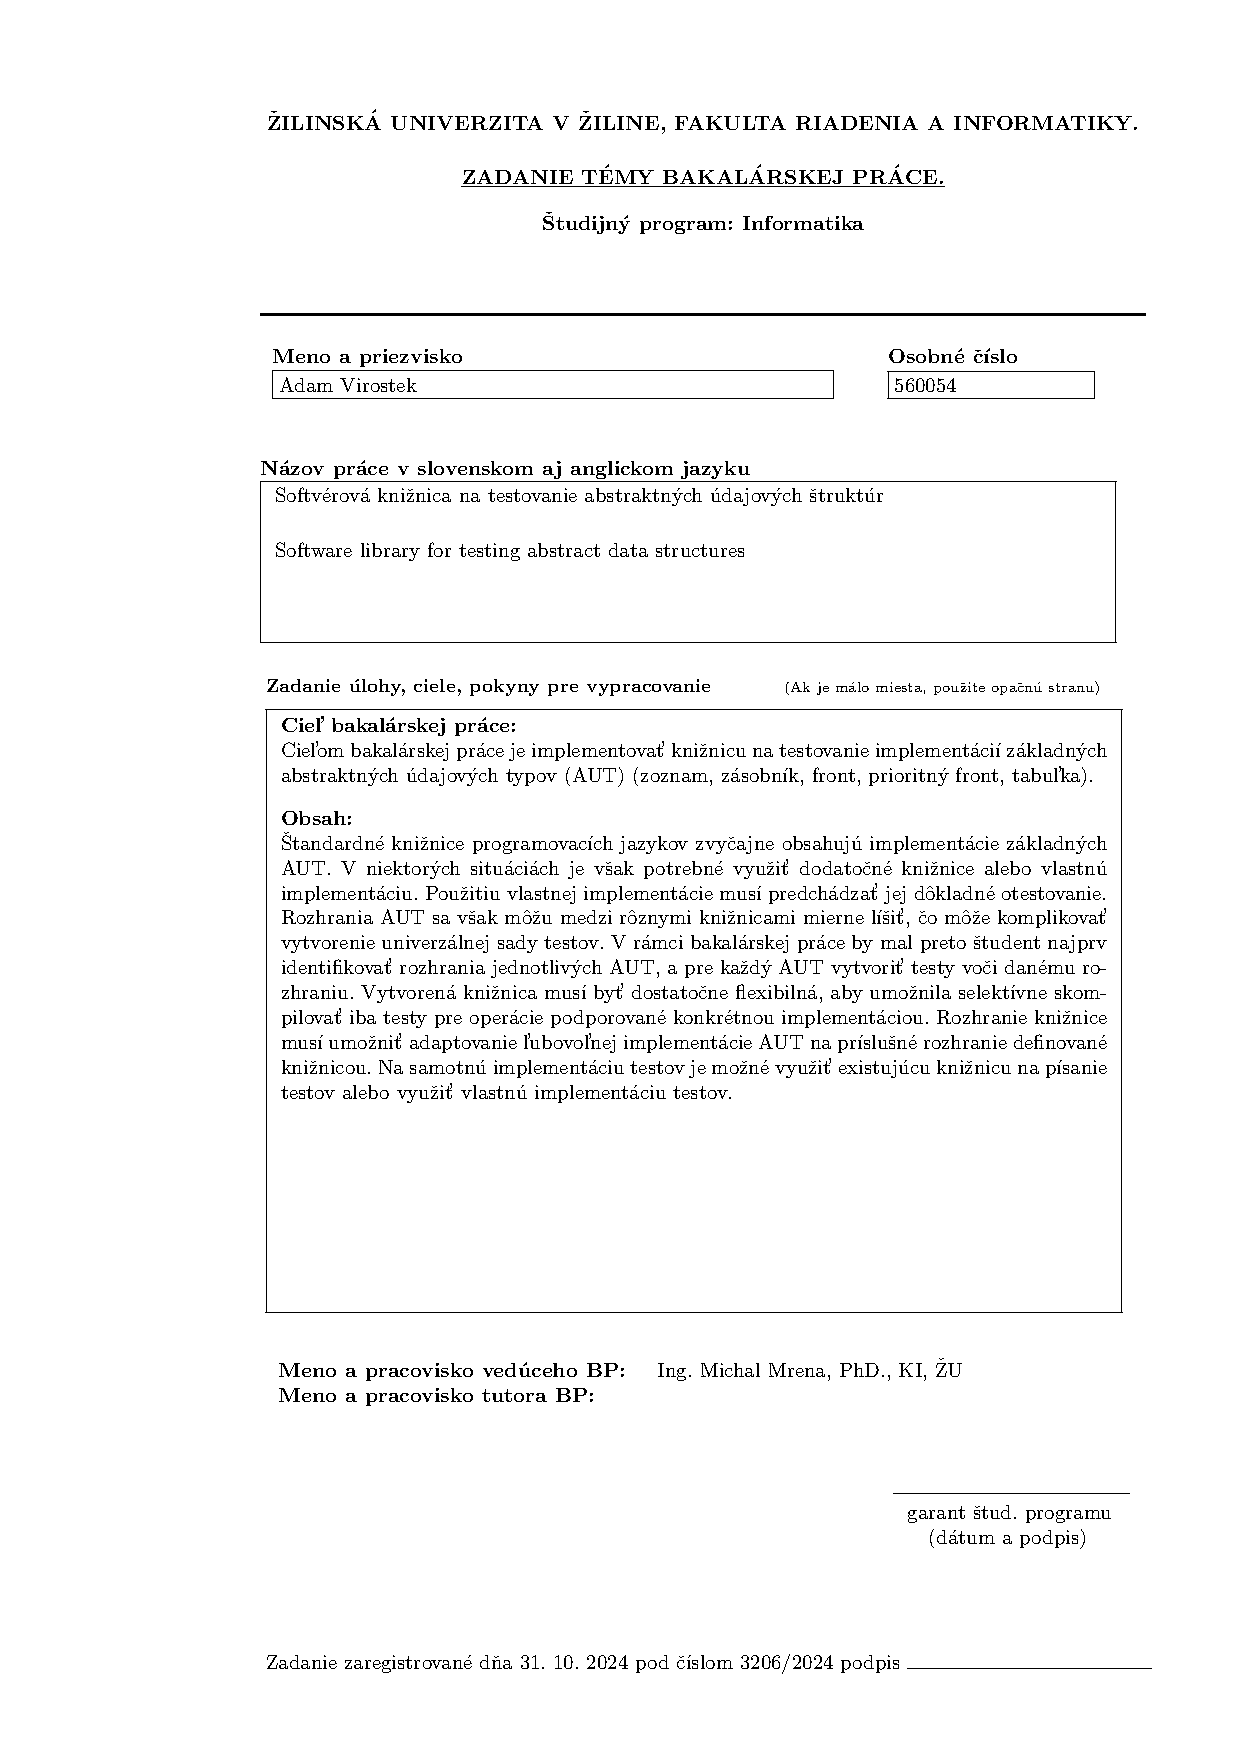
\includepdf[pages=-,offset=-30 0]{zadanie.pdf}

\newpage

\vspace*{\fill}
\begin{flushleft}
  \Large\bfseries Čestné vyhlásenie
\end{flushleft}
\vspace{0.5cm}
\noindent Vyhlasujem, že som zadanú bakalársku prácu vypracoval samostatne, pod odborným vedením vedúceho práce a používal som len literatúru uvedenú v práci.\par
\vspace{1cm}
\noindent Žilina, 28. Apríla 2025 \hfill \textit{podpis}

\newpage

\vspace*{\fill}
\begin{flushleft}
  \Large\bfseries Poďakovanie
\end{flushleft}
\vspace{0.5cm}
\noindent Moje veľké poďakovanie patrí vedúcemu bakalárskej práce Ing. Michalovi Mrenovi, PhD. za odbornú pomoc, za dôveru, motiváciu a cenné pripomienky pri tvorbe tejto práce.\par

\newpage

% --- Abstrakt a Kľúčové slová ---
\begin{abstract}

  \noindent
  Adam Virostek: Softvérová knižnica na testovanie abstraktných údajových štruktúr. [Bakalárska práca]. -- Žilinská Univerzita v Žiline, Fakulta riadenia a informatiky, Katedra informatiky. -- Školiteľ: Ing. Michal Mrena, PhD. -- Stupeň odbornej kvalifikácie: bakalár. -- FRI ŽU v Žiline, 2025. -- \pageref*{LastPage} s.

  \bigskip
  Táto bakalárska práca sa zaoberá návrhom a implementáciou univerzálnej knižnice na testovanie údajových štruktúr v jazyku C++. Knižnica je navrhnutá tak, aby poskytovala efektívne a flexibilné nástroje na testovanie implementácií základných abstraktných údajových typov (AUT), ako sú zoznam, zásobník, front, prioritný front a tabuľka. Práca sa zameriava na overenie správnosti implementácie testovanej údajovej štruktúry a jej efektívnosti pri spracovaní veľkých objemov dát. Dôraz je kladený na univerzálnosť knižnice, aby ju bolo možné použiť pre širokú škálu C++ implementácií údajových štruktúr.
  \bigskip

  \noindent\textbf{Kľúčové slová:} Abstraktné Údajové Typy, Algoritmy, C++, Knižnica, Testovanie, Údajové štruktúry
\end{abstract}

\newpage

\begin{english}
  \begin{abstract}

    \noindent
    Adam Virostek: Software library for testing abstract data structures. [Bachelor thesis]. -- University of Žilina, Faculty of Management Science and Informatics, Department of Informatics. -- Advisor: Ing. Michal Mrena, PhD. -- Qualification level: Bachelor's degree. -- FRI ŽU in Žilina, 2025. -- \pageref*{LastPage} s.

    \bigskip
    This bachelor thesis deals with the design and implementation of a universal library for testing data structures in C++. The library is designed to provide efficient and flexible tools for testing implementations of basic abstract data types (ADTs), such as list, stack, queue, priority queue, and table. The work focuses on verifying the correctness of the tested data structure implementation and its efficiency when processing large volumes of data. The library is implemented with an emphasis on universality, allowing it to be used for a wide range of C++ data structure implementations.
    \bigskip

    \noindent\textbf{Keywords:} Abstract Data Types, Algorithms, C++, Data Structures, Library, Testing
  \end{abstract}
\end{english}

\newpage

% --- Obsah, Zoznamy ---
\tableofcontents
\newpage
\listoffigures
\newpage
\listoftables
\newpage
\lstlistoflistings
\newpage

% --- Zoznam skratiek ---
\section*{Zoznam skratiek}
\begin{table}[H]
  \centering
  \begin{tabularx}{\textwidth}{>{\raggedright\arraybackslash}X>{\raggedright\arraybackslash}X}
   \toprule
   \textbf{Skratka} & \textbf{Význam} \\
   \midrule
   ADTs & Abstract Data Types (anglický ekvivalent AUT) \\
   \midrule
   API & Application Programming Interface \\
   \midrule
   APS & Abstraktná pamäťová štruktúra \\
   \midrule
   AUS & Abstraktná údajová štruktúra \\
   \midrule
   AUT & Abstraktný Údajový Typ \\
   \midrule
   BDD & Behavior-Driven Development \\
   \midrule
   BFS & Breadth-First Search (Prehľadávanie do šírky) \\
   \midrule
   BVS & Binárny vyhľadávací strom \\
   \midrule
   FIFO & First-In, First-Out \\
   \midrule
   GMock & Google Mock \\
   \midrule
   GTest & Google Test \\
   \midrule
   LIFO & Last-In, First-Out \\
   \midrule
   OS & Operačný Systém \\
   \midrule
   SFINAE & Substitution Failure Is Not An Error \\
   \midrule
   STL & Standard Template Library \\
   \bottomrule
  \end{tabularx}
  \caption{Zoznam použitých skratiek}
  \label{tab:skratky}
 \end{table}

\newpage

% --- Úvod ---
\section*{Úvod}
\addcontentsline{toc}{section}{\protect\numberline{}Úvod}
Implementácia a testovanie údajových štruktúr predstavujú kľúčovú oblasť informatických vied a softvérového inžinierstva. Údajové štruktúry, akými sú zoznamy, zásobníky, fronty, prioritné fronty či tabuľky, zohrávajú nezastupiteľnú úlohu pri navrhovaní efektívnych algoritmických riešení. Predstavujú základné stavebné bloky, ktoré umožňujú uchovávať, spracovávať a organizovať údaje spôsobom, ktorý zohľadňuje výpočtovú náročnosť a optimalizuje výkonnosť celého softvérového systému. Ich implementácia je bežnou súčasťou mnohých softvérových projektov, či už v akademickom alebo komerčnom prostredí.

Spoľahlivosť týchto fundamentálnych štruktúr má priamy dopad na stabilitu a funkčnosť celého softvérového riešenia. Korektnosť ich správania je preto kritickým faktorom, najmä pri práci s veľkými objemami údajov, kde aj zdanlivo malá implementačná chyba môže viesť k závažným problémom, ako sú strata dát, chybné výpočty alebo celková nestabilita systému. Napriek ich dôležitosti sa v akademickej sfére testovanie implementácií údajových štruktúr často podceňuje alebo sa realizuje len formálne. Bežnou praxou je použitie jednoduchých testov, ktoré overujú iba základné prípady použitia, zatiaľ čo zložitejšie scenáre, hraničné prípady (tzv. "edge cases") či správanie pri nevalidných vstupoch bývajú opomínané. Dôsledkom tohto prístupu vo výučbe je, že študenti síce často zvládnu implementačný aspekt údajových štruktúr, avšak nemajú dostatočne rozvinuté návyky v oblasti ich dôsledného a systematického testovania.

Dôsledné testovanie implementácií základných abstraktných údajových typov (AUT) -- ako sú zoznam, zásobník, front, prioritný front a tabuľka -- je nevyhnutným predpokladom pre zabezpečenie korektnosti a spoľahlivosti softvérových systémov. Tieto údajové štruktúry sú často implementované buď vo forme vlastných riešení, alebo prostredníctvom externých či štandardných knižníc, akými sú napríklad Standard Template Library (STL) v jazyku C++ alebo Java Collections Framework v jazyku Java. Táto rôznorodosť implementácií prirodzene vytvára potrebu ich jednotného a systematického overovania.

Ďalšiu výzvu predstavuje heterogenita rozhraní (API) pre rovnaké AUT v rámci štandardných knižníc rôznych programovacích jazykov, ako sú Java, Rust či C++. Odlišné konvencie a prístupy k práci s týmito typmi sťažujú vytvorenie univerzálneho testovacieho mechanizmu. Preto sme sa rozhodli navrhnúť riešenie, ktoré by umožnilo efektívne a konzistentné overovanie správnosti implementácií AUT, ideálne nezávisle od ich konkrétneho pôvodu či špecifík danej knižnice alebo programovacieho jazyka.

Z praktického hľadiska síce súčasné testovacie frameworky, ako napríklad Google Test alebo Catch2, poskytujú robustné nástroje na tvorbu jednotkových testov, avšak neponúkajú explicitnú podporu pre testovanie špecifických aspektov údajových štruktúr. Chýbajú nástroje pre jednoduché definovanie a overovanie komplexných sekvencií operácií, testovanie invariantov údajových štruktúr či ich výkonnostných charakteristík. Vytváranie takýchto špecializovaných testov je často časovo náročné a vyžaduje si manuálnu konfiguráciu, čo obmedzuje ich širšie použitie.

Z vyššie uvedených dôvodov vyplýva nevyhnutnosť existencie špecializovanej knižnice, ktorá by podporovala testovanie údajových štruktúr na úrovni ich abstraktného správania -- teda nezávisle od konkrétnej implementácie, použitých dátových typov (v rámci možností generického programovania) alebo špecifických jazykových konvencií. Takáto knižnica by mala byť flexibilná, ľahko rozšíriteľná, konfigurovateľná a schopná využívať moderné programovacie techniky, ako napríklad koncepty pridané do štandardnej knižnice v štandarde C++20, na automatickú detekciu podporovaných operácií testovanej štruktúry.

Primárnym cieľom tejto bakalárskej práce je preto návrh a implementácia knižnice určenej na testovanie implementácií základných abstraktných údajových typov v jazyku C++. Navrhovaná knižnica má slúžiť ako nezávislý testovací nástroj, ktorý umožní overenie funkčnej korektnosti rôznych implementácií AUT (napr. zo štandardnej knižnice, externých knižníc alebo vlastných implementácií) prostredníctvom jednotného a konzistentného rozhrania. Medzi kľúčové požiadavky kladené na túto knižnicu patria:

\begin{itemize}
  \item \textbf{Univerzálnosť v rámci C++:} Schopnosť testovať rôzne C++ implementácie AUT (šablónové aj nešablónové) pochádzajúce z rôznych zdrojov (STL, Boost, vlastné riešenia) pomocou spoločného testovacieho frameworku.
  \item \textbf{Selektívna kompilácia testov:} Využitie moderných C++ techník (napr. koncepty a type traits) na kompiláciu iba tých testov, ktorých operácie testovaná štruktúra skutočne podporuje, čím sa optimalizuje čas kompilácie.
\end{itemize}

Výber tejto témy je motivovaný snahou prepojiť teoretické poznatky z oblasti údajových štruktúr s praktickými potrebami softvérového vývoja, konkrétne s problematikou zabezpečenia kvality kódu. Výsledná knižnica má ambíciu stať sa praktickým nástrojom nielen pre vývojárov a pedagógov v oblasti informatiky, ale aj projektom s voľne dostupným zdrojovým kódom (open-source). Hlavným prínosom práce má byť možnosť jednotného, opakovateľného a čiastočne automatizovaného overovania správnosti implementácií AUT cez spoločné rozhranie, čo by malo znížiť časové aj vývojové náklady spojené s tvorbou špecifických testov pre každú implementáciu. Tento nástroj môže nájsť uplatnenie v akademickej sfére ako pomôcka pri výučbe a overovaní študentských prác, ako aj v praxi ako podpora pre vývojárov pri zabezpečovaní kvality kritických komponentov softvérových systémov.

Nasledujúce kapitoly tejto práce sa venujú analýze existujúcich prístupov k testovaniu údajových štruktúr, opisu základných údajových typov a ich implementácií, detailnému návrhu architektúry a rozhraní vyvíjanej knižnice. Nakoniec opisu jej implementácie s využitím moderných C++ prvkov a napokon zhodnoteniu dosiahnutých výsledkov a možnostiam ďalšieho rozvoja.

% --- Analýza ---
\newpage
\section{Analýza} \label{sec:analyza}

Pred samotným návrhom a implementáciou testovacej knižnice je nevyhnutné dôsledne vymedziť základnú terminológiu, objasniť relevantné technológie a vykonať analýzu existujúcich riešení v danej oblasti. Kľúčovou požiadavkou na efektívnu knižnicu pre testovanie údajových štruktúr je schopnosť spoľahlivo a presne validovať korektnosť implementácií širokého spektra abstraktných údajových typov (AUT).

V odbornej literatúre nachádzame viaceré prístupy k riešeniu tejto problematiky. Napríklad, Del Vado Vírseda a Morente \cite{VIIRSEDA20121743} predstavili edukačný nástroj využívajúci algebraické špecifikácie, ktorý umožňuje overenie sémantickej správnosti AUT bez nutnosti znalosti konkrétnej implementácie. Hoci sú tieto formálne metódy robustné, ich praktická aplikácia môže byť pre štandardného vývojára zložitá a menej intuitívna. Sutton a Zalewski \cite{6405251} upozorňujú na nedostatok adekvátnej podpory pre testovanie generických a šablónových dátových štruktúr v dostupných nástrojoch, čo predstavuje signifikantnú výzvu najmä v kontexte jazyka C++. Navrhovaná knižnica reaguje na tieto identifikované nedostatky poskytnutím praktického a flexibilného riešenia, ktoré je špecificky zamerané na testovanie C++ implementácií, vrátane generických typov, s primárnym dôrazom na jednoduchosť použitia a vysokú mieru automatizácie. Potrebu pokročilých testovacích techník zdôrazňujú aj Bonfanti a Gargantini \cite{8411752}, ktorí poukazujú na výhody generovania testovacích prípadov z abstraktných stavových modelov pre redukciu chýb v softvérových projektoch využívajúcich C++.

Táto kapitola sa preto zameriava na podrobnú analýzu kľúčových aspektov nevyhnutných pre návrh: použitého programovacieho jazyka (C++), relevantných štandardných knižníc (STL), povahy samotných abstraktných údajových typov a prehľadu existujúcich metód k ich testovaniu.

\subsection{Abstraktné Údajové Typy a ich implementácie}

Abstraktné údajové typy (AUT) patria medzi základné oblasti informatiky a programovania, slúžia ako základné stavebné bloky pre návrh a implementáciu efektívnych algoritmov a údajových štruktúr. Kľúčovým aspektom AUT je ich zameranie na definíciu logického správania a súboru operácií nad údajmi (doménou prvkov), pričom abstrahujú od konkrétnych detailov implementácie \cite{aus3}. Údajová štruktúra je potom konkrétny spôsob organizácie a ukladania dát, ktorý realizuje špecifikácie daného AUT \cite{aus3}. AUT je teda možné realizovať viacerými abstraktnými údajovými štruktúrami (AUS) \cite{aus3}. Samotné AUS využívajú na ukladanie prvkov v pamäti zodpovedajúce abstraktné pamäťové štruktúry (APS), ktoré definujú organizáciu blokov pamäte a požiadavky na správcu pamäte \cite{aus2}. Voľba vhodnej AUS a jej podkladovej APS závisí od požadovaných operácií a očakávanej početnosti ich volaní s cieľom minimalizovať časové a pamäťové nároky \cite{aus2}. Hlboké porozumenie týmto konceptom, ako aj ich bežným implementáciám, napríklad v rámci C++ Standard Template Library (STL), je esenciálne. Táto kapitola sa venuje podrobnému opisu piatich kľúčových abstraktných údajových typov, ktoré sú neoddeliteľnou súčasťou algoritmického spracovania údajov:

\subsubsection{Zoznam (List)}

Definuje sa ako lineárna sekvencia alebo kolekcia prvkov, kde každý prvok (s výnimkou prvého a posledného) má práve jedného predchodcu a jedného nasledovníka \cite{aus2}. Umožňuje dynamické operácie ako vkladanie, odstraňovanie a prístup k prvkom, často na základe indexu. Bežné implementácie (AUS) vychádzajú z APS typu Sekvencia (Sequence) \cite{aus2}. Patrí sem implicitná sekvencia (realizovaná typicky poľom v súvislej pamäti) \cite{aus2}, ktorá umožňuje efektívny prístup k prvkom cez index ($O(1)$), ale pomalšie modifikácie v strede ($O(n)$) \cite{aus2}. Ďalej sem patria explicitné sekvencie, ako jednostranne (singly linked) alebo obojstranne zreťazené (doubly linked) zoznamy \cite{aus2}, ktoré umožňujú efektívnejšie vkladanie a odstraňovanie prvkov ($O(1)$ pri známom susedovi), ale prístup k prvku na základe indexu môže byť pomalší ($O(n)$) \cite{aus2}. Implementácie môžu byť aj cyklické \cite{aus2}. V C++ STL zodpovedajú týmto konceptom napr. std::vector (implicitná sekvencia) a std::list, std::forward\_list (explicitné sekvencie).

\subsubsection{Zásobník (Stack)}

Tento AUT je charakterizovaný princípom LIFO (Last-In, First-Out), čo znamená, že naposledy vložený prvok je odstránený ako prvý \cite{aus3}. Priorita prvku je implicitná, daná časom vloženia \cite{aus3}. Základné operácie sú Vlož (push), Vyber (pop) a Vrchol (top alebo peek) \cite{aus3}. Operácie sa vykonávajú na rovnakom konci sekvencie \cite{aus3}. Zásobníky nachádzajú uplatnenie pri spracovaní rekurzie, vyhodnocovaní výrazov a algoritmoch spätného sledovania (backtracking). Implementácie (AUS) môžu byť založené na implicitnej sekvencii (Implicitný zásobník) s operáciami na konci ($O(1)$ amortizovane pre vloženie/vybratie) alebo explicitnej jednostranne zreťazenej sekvencii (Explicitný zásobník) s operáciami na začiatku ($O(1)$) \cite{aus3}. V C++ sa často realizuje ako adaptér std::stack nad iným kontajnerom.

\subsubsection{Front (Queue)}

Front funguje na princípe FIFO (First-In, First-Out), kde prvok, ktorý bol vložený ako prvý, je aj ako prvý odstránený \cite{aus3}. Priorita prvku je implicitná, daná časom vloženia \cite{aus3}. Typické operácie sú Vlož (enqueue), Vyber (dequeue) a Vrchol (front) \cite{aus3}. Vkladanie a vyberanie prebieha na opačných koncoch sekvencie \cite{aus3}. Používa sa v oblastiach ako plánovanie procesov, správa úloh, simulácie a prehľadávanie grafov do šírky (BFS). Efektívna implementácia pomocou implicitnej sekvencie vyžaduje cyklickú štruktúru s fixnou kapacitou (Implicitný front), aby sa predišlo neefektívnemu posúvaniu prvkov \cite{aus3}. Explicitný front typicky využíva jednostranne zreťazenú sekvenciu s referenciou na prvý aj posledný prvok, aby boli operácie Vlož (na koniec) aj Vyber/Vrchol (zo začiatku) efektívne ($O(1)$) \cite{aus3}. V C++ sa často realizuje ako adaptér std::queue.

\subsubsection{Prioritný front (Priority Queue)}

Ide o modifikáciu frontu, kde každý prvok má priradenú explicitnú prioritu (alebo implicitnú v špeciálnych prípadoch ako zásobník a front) \cite{aus3}. Operácia Vyber odstraňuje prvok s najvyššou prioritou (podľa definovaného usporiadania priorít), bez ohľadu na poradie vloženia \cite{aus3}. Kľúčové operácie sú Vlož (prvok s prioritou), Vyber (prvok s najvyššou prioritou) a Vrchol (náhľad na prvok s najvyššou prioritou) \cite{aus3}. Sekvenčné implementácie (utriedené alebo neutriedené) majú zvyčajne aspoň jednu operáciu s lineárnou zložitosťou ($O(n)$), a preto nie sú veľmi efektívne \cite{aus3}. Efektívnejšie implementácie zahŕňajú Dvojzoznam (kombinácia krátkej utriedenej a dlhej neutriedenej sekvencie, amortizovaná zložitosť $O(\sqrt{n})$ alebo $O(m)$, kde $m$ je dĺžka krátkej sekvencie) \cite{aus3} alebo štruktúry založené na hierarchiách, ako je Ľavostranná halda (implementovaná pomocou implicitnej binárnej hierarchie), ktorá dosahuje logaritmickú zložitosť operácií Vlož a Vyber ($O(\log n)$) \cite{aus3}. V C++ STL je implementovaný ako std::priority\_queue, typicky pomocou haldy.

\subsubsection{Tabuľka (Table/Map/Dictionary)}

Predstavuje asociatívnu údajovú štruktúru, ktorá ukladá páry kľúč-hodnota a umožňuje efektívny prístup k hodnotám (prvkom) na základe ich unikátnych kľúčov. Základné operácie zahŕňajú Vlož, Nájdi (alebo Skús nájsť pre bezpečnejší prístup), Obsahuje a Vyber \cite{aus3}. Implementácie sa líšia:
  \begin{itemize}
    \item Sekvenčné tabuľky: Ukladajú prvky do sekvencie (implicitnej alebo explicitnej). Môžu byť neutriedené (vyhľadávanie $O(n)$, vloženie $O(1)$ bez kontroly unikátnosti) alebo utriedené (vyhľadávanie $O(\log n)$ pri použití implicitnej sekvencie a polenia intervalov, vloženie/vymazanie $O(n)$) \cite{aus3}.
    \item Tabuľka s rozptýlenými záznamami (Hash Table): Využíva hešovaciu funkciu na mapovanie kľúčov na indexy v implicitnej sekvencii (poli) \cite{aus3}. Priemerne dosahuje konštantnú zložitosť ($O(1)$) pre základné operácie \cite{aus3}, ale vyžaduje riešenie kolízií (napr. zreťazovaním) \cite{aus3}. V C++ implementované ako std::unordered\_map.
    \item Binárny vyhľadávací strom (Binary Search Tree - BVS): Hierarchická štruktúra udržiavajúca usporiadanie podľa kľúčov \cite{aus3}. Priemerne dosahuje logaritmickú zložitosť ($O(\log n)$), ale v najhoršom prípade (nevyvážený strom) degeneruje na lineárnu ($O(n)$) \cite{aus3}. Existujú samovyvažovacie varianty (napr. AVL stromy, červeno-čierne stromy, Treap \cite{aus3}), ktoré garantujú logaritmickú zložitosť aj v najhoršom prípade. V C++ implementované ako std::map (typicky červeno-čierny strom).
  \end{itemize}

Správny výber a efektívna implementácia týchto základných abstraktných údajových typov má zásadný dopad na výkonnosť, škálovateľnosť a spoľahlivosť softvérových systémov.

\subsubsection{Údajové štruktúry}

Údajová štruktúra predstavuje formálny objekt, ktorý slúži na agregáciu údajov a poskytuje definovaný súbor operácii na ich spracovanie. Každá údajová štruktúra má svoje vlastnosti a podporuje operácie, ktoré umožňujú efektívnu manipuláciu s uchovávanými údajmi. Z hľadiska efektívneho riešenia konkrétnej úlohy má používateľ (programátor) dve základné úlohy \cite{prednaska_aus1}:

\begin{itemize}
  \item Na základe požadovaných operácii nad údajmi identifikovať a zvoliť vhodný typ údajovej štruktúry (napríklad zoznam, zásobník, front, prioritný front, tabuľku, strom a pod.).
  \item S ohľadom na očakávanú početnosť jednotlivých operácii zvoliť optimálnu implementáciu vybranej štruktúry, ktorá minimalizuje časovú a pamäťovú náročnosť pri danom spôsobe použitia.
\end{itemize}

Cieľom je navrhnúť taký model údajovej reprezentácie a manipulácie, ktorý bude z pohľadu využívania pamäťových prostriedkov úsporný a zároveň zabezpečí vysokú efektivitu (predovšetkým rýchlosť) často vykonávaných algoritmických operácii \cite{aus1}.

\subsubsection*{Kategorizácia operácii nad údajovými štruktúrami}

Operácie realizované nad údajovými štruktúrami je možné klasifikovať nasledovne:

\begin{itemize}
  \item Základné operácie -- operácie slúžiace na vytváranie a likvidáciu štruktúr (konštruktory, deštruktory), ako aj priradenie a porovnávanie štruktúr \cite{aus3}.
  \item Selektory -- operácie umožňujúce vyhľadávanie alebo sprístupnenie konkrétnych prvkov v rámci štruktúry \cite{aus3}.
  \item Dotazy -- poskytujú informácie o jednotlivých prvkoch alebo o vlastnostiach štruktúry ako celku (napr. počet prvkov, prázdnosť, kapacita a pod.) \cite{aus3}.
  \item Modifikátory -- operácie umožňujúce pridávanie, odstraňovanie alebo úpravu prvkov, čím menia obsah údajovej štruktúry \cite{aus3}.
  \item Prehliadky -- sprístupňujú všetky prvky v štruktúre v určenom poradí. Ich realizácia môže byť zapúzdrená do samostatných objektov (tzv. iterátorov), ktoré umožňujú efektívny prístup k prvkom bez odhalenia detailov implementácie samotnej štruktúry \cite{aus3}.
\end{itemize}

\subsubsection{Analýza rozhraní údajových štruktúr}

Pre vytvorenie univerzálnej testovacej knižnice pre údajové štruktúry je potrebné analyzovať rôzne implementácie základných AUT v rôznych programovacích jazykoch a ich prístupy k testovaniu údajových štruktúr. Tento proces je kľúčový pre pochopenie, ako rôzne jazyky a technológie pristupujú k manipulácii s údajmi v rôznych kontextoch.:

\subsubsection*{Zoznam (List)}

\begin{itemize}
  \item \textbf{C++:} Štandardná knižnica (STL) ponúka std::list a std::vector.
  \begin{itemize}
    \item std::list je implementovaná ako obojstranne zreťazený zoznam \cite{c++_containers}.
    Výhody: Konštantný čas $O(1)$ na vkladanie a vymazávanie na ľubovoľnej pozícii pomocou iterátora.
    Nevýhody: Pomalý prístup k prvkom podľa indexu ($O(n)$), vyššia pamäťová náročnosť kvôli ukazovateľom v každom uzle.
    \item std::vector je implementovaná ako implicitná sekvencia \cite{c++_containers}.
    Výhody: Rýchly prístup k prvkom podľa indexu ($O(1)$).
    Nevýhody: Vkladanie a vymazávanie v strede alebo na začiatku zoznamu môže byť pomalé ($O(n)$ kvôli presunu prvkov), realokácia pamäte pri prekročení kapacity.
  \end{itemize}
  \item \textbf{C:} Jazyk C neposkytuje vstavaný typ pre zoznam, preto je potrebné implementovať ho manuálne, typicky pomocou štruktúr a ukazovateľov na vytvorenie zreťazeného zoznamu.
  Výhody: Maximálna flexibilita a kontrola nad alokáciou pamäte.
  Nevýhody: Vysoké riziko chýb pri práci s ukazovateľmi a manuálnou správou pamäte, nutnosť ručne implementovať všetky operácie.
  \item \textbf{C\#:} .NET Framework poskytuje System.Collections.Generic.List<T> a System.Collections.Generic.LinkedList<T>.
  \begin{itemize}
    \item List<T> je implicitná sekvencia \cite{dotnet_docs}. Výhody: Rýchly prístup podľa indexu ($O(1)$), dobrý výkon pri pridávaní na koniec. Nevýhody: Pomalé vkladanie a mazanie v strede/na začiatku ($O(n)$).
    \item LinkedList<T> je implementovaný ako obojstranne zreťazený zoznam \cite{dotnet_docs}. Výhody: Efektívne vkladanie a odstraňovanie na ľubovoľnej pozícii ($O(1)$). Nevýhody: Pomalý prístup podľa indexu ($O(n)$), vyššie pamäťové nároky.
  \end{itemize}
  \item \textbf{Java:} Java Collections Framework poskytuje rozhranie List s niekoľkými implementáciami, najčastejšie ArrayList<T> a LinkedList<T>.
  \begin{itemize}
    \item ArrayList<T> je implementovaný ako implicitná sekvencia \cite{java_docs}. Výhody: Rýchly prístup podľa indexu ($O(1)$). Nevýhody: Pomalé vkladanie a mazanie inde ako na konci ($O(n)$).
    \item LinkedList<T> implementuje rozhrania List a Deque a je implementovaný ako obojstranne zreťazený zoznam \cite{java_docs}. Výhody: Efektívne vkladanie a odstraňovanie na oboch koncoch a v strede ($O(1)$ po získaní iterátora). Nevhody: Pomalý prístup podľa indexu ($O(n)$).
  \end{itemize}
  \item \textbf{Rust:} Rust Standard Library poskytuje Vec<T> a LinkedList<T> \cite{rust_collections}.
  \begin{itemize}
    \item Vec<T> je implicitná sekvencia \cite{rust_collections}. Výhody: Rýchly prístup podľa indexu ($O(1)$), efektívne pridávanie/odstraňovanie na konci ($O(1)$ amortizovane). Nevýhody: Pomalé vkladanie/odstraňovanie v strede/na začiatku ($O(n)$).
    \item LinkedList<T> je obojstranne zreťazený zoznam \cite{rust_collections}. Výhody: $O(1)$ vkladanie a odstraňovanie na oboch koncoch. Nevýhody: $O(n)$ prístup k prvkom, vyššia pamäťová náročnosť. Rust tiež poskytuje VecDeque<T>, ktorý je cyklický obojsmerný front (\textit{double-ended queue}) a môže slúžiť ako efektívnejšia alternatíva k LinkedList pre niektoré operácie na oboch koncoch ($O(1)$).
  \end{itemize}
\end{itemize}

\subsubsection*{Zásobník (Stack)}

\begin{itemize}
  \item \textbf{C++:} Štandardná knižnica poskytuje std::stack, ktorý je adaptérom pre iné kontajnery (predvolene std::deque, možno použiť aj std::vector alebo std::list) \cite{c++_containers}. Poskytuje LIFO (Last-In, First-Out) funkcionalitu.
  Výhody: Jednoduché a bezpečné API obmedzené na operácie push, pop, top. Výkon závisí od podkladového kontajnera, ale pre std::deque a std::vector sú operácie $O(1)$.
  Nevýhody: Obmedzené len na základné operácie zásobníka.
  \item \textbf{C:} Zásobník sa implementuje manuálne, zvyčajne pomocou sekvencie.
  Výhody: Úplná kontrola nad implementáciou a pamäťou.
  Nevýhody: Vyžaduje starostlivú manuálnu správu pamäte a implementáciu všetkých operácií, vyššie riziko chýb.
  \item \textbf{C\#:} .NET Framework poskytuje vstavanú generickú triedu System.Collections.Generic.Stack<T> \cite{dotnet_docs}. Implementovaná je na báze implicitnej sekvencie.
  Výhody: Rýchle LIFO operácie (Push, Pop, Peek) s výkonom $O(1)$ amortizovane pre Push. Generická podpora pre typy.
  Nevýhody: Pri prekročení kapacity poľa dochádza k realokácii, čo môže mať v ojedinelých prípadoch vyššiu časovú náročnosť.
  \item \textbf{Java:} Java Collections Framework poskytuje triedu Stack, ktorá dedí od Vector \cite{java_docs}. Hoci sa dá použiť, preferovaným spôsobom implementácie zásobníka v modernej Jave je použitie rozhrania Deque (napr. s implementáciou ArrayDeque alebo LinkedList), ktoré poskytuje robustnejšie a konzistentnejšie API pre operácie na oboch koncoch \cite{java_docs}.
  Výhody: Jednoduché API pre LIFO operácie.
  Nevýhody: Trieda Stack je považovaná za menej efektívnu v porovnaní s Deque implementáciami, Vector je synchronizovaný, čo môže byť zbytočná réžia v jedno-vláknových aplikáciách.
  \item \textbf{Rust:} Rust používa Vec<T> na implementáciu zásobníka pomocou metód push a pop. Tieto operácie sú efektívne s amortizovaným časom $O(1)$ \cite{rust_collections}.
  Výhody: Využíva efektívnu implementáciu implicitnej sekvencie v Ruste, pamäťová bezpečnosť zabezpečená kompilátorom.
  Nevýhody: Vec je všeobecné implicitná sekvencia, prístup k prvkom nie je striktne obmedzený len na LIFO operácie, ak sa explicitne nevynúti.
\end{itemize}

\subsubsection*{Front (Queue)}

\begin{itemize}
  \item \textbf{C++:} Štandardná knižnica ponúka std::queue, ktorá je adaptérom pre iné kontajnery (predvolene std::deque, možno použiť aj std::list) \cite{c++_containers}. Poskytuje FIFO (First-In, First-Out) funkcionalitu.
  Výhody: Jednoduché a bezpečné API obmedzené na operácie push (pridanie na koniec) a pop (odstránenie zo začiatku), front (prístup k prvému prvku). Výkon závisí od podkladového kontajnera, pre std::deque a std::list sú tieto operácie $O(1)$.
  Nevýhody: Obmedzené len na základné operácie frontu.
  \item \textbf{C:} Implementácia frontu je zvyčajne manuálna, pomocou implicitných sekvencií (s cyklickým bufferom pre efektivitu).
  Výhody: Úplná kontrola. Flexibilita v správe pamäte.
  Nevýhody: Potreba ručne spravovať alokáciu/dealokáciu pamäte a indexy, vyššie riziko chýb.
  \item \textbf{C\#:} .NET Framework poskytuje generický System.Collections.Generic.Queue<T> \cite{dotnet_docs}. Implementovaný je na báze cyklického poľa.
  Výhody: Efektívne FIFO operácie (Enqueue, Dequeue, Peek) s výkonom $O(1)$ amortizovane pre Enqueue.
  Nevýhody: Obmedzený prístup k prvkom okrem prvého. Pri realokácii poľa môže nastať vyššia časová náročnosť.
  \item \textbf{Java:} Java Collections Framework má rozhranie Queue s implementáciami ako LinkedList a ArrayDeque \cite{java_docs}. ArrayDeque je typicky preferovaná pre implementáciu frontu vďaka svojej efektivite.
  Výhody: Jednoduché API pre FIFO operácie, ArrayDeque poskytuje $O(1)$ amortizovaný čas pre pridávanie a odstraňovanie na oboch koncoch.
  Nevýhody: Výkon sa môže líšiť v závislosti od implementácie (LinkedList má vyššiu pamäťovú réžiu).
  \item \textbf{Rust:} Rust používa VecDeque<T> na implementáciu frontu. VecDeque je cyklický obojsmerný front a poskytuje efektívne operácie pridávania a odstraňovania na oboch koncoch ($O(1)$ amortizovane) \cite{rust_collections}.
  Výhody: Efektívne FIFO operácie vďaka optimalizovanej dátovej štruktúre, pamäťová bezpečnosť.
  Nevýhody: O niečo vyššia pamäťová náročnosť v porovnaní s jednoduchým poľom kvôli obojsmernej povahe.
\end{itemize}

\subsubsection*{Prioritný front (Priority Queue)}

\begin{itemize}
  \item \textbf{C++:} Štandardná knižnica ponúka triedu std::priority\_queue, ktorá využíva binárnu haldu (max-heap v predvolenom nastavení) implementovanú pomocou iného kontajnera (predvolene std::vector) \cite{c++_containers}.
  Výhody: Rýchly prístup k prvku s najvyššou prioritou (top $O(1)$). Operácie vkladania (push) a odstraňovania najvyššieho prvku (pop) majú logaritmickú časovú náročnosť ($O(\log n)$). Podpora pre rôzne porovnávacie funkcie na definovanie priority.
  Nevýhody: Priamy prístup k prvkom okrem najvyššieho nie je efektívny, odstraňovanie ľubovoľného prvku je zložité.
  \item \textbf{C:} Implementácia prioritného frontu je často realizovaná manuálne pomocou binárnej haldy alebo iných stromových štruktúr.
  Výhody: Úplná kontrola nad dátovou štruktúrou a jej optimalizáciou pre špecifické použitie.
  Nevýhody: Komplexná manuálna správa pamäte a implementácia haldových operácií, vysoké riziko chýb.
  \item \textbf{C\#:} .NET Framework poskytuje od .NET 6 generickú triedu System.Collections.Generic.PriorityQueue<TElement, TPriority> \cite{dotnet_docs}. Implementovaná je na báze binárnej haldy.
  Výhody: Efektívne operácie Enqueue (vloženie) a Dequeue (odstránenie s najvyššou prioritou) s časovou náročnosťou $O(\log n)$. Podporuje definovanie priority pomocou samostatného typu a komparátora.
  Nevýhody: Podobne ako v C++, priamy prístup k prvkom inej priority nie je efektívny.
  \item \textbf{Java:} Java Collections Framework poskytuje triedu PriorityQueue, ktorá implementuje rozhranie Queue a využíva binárnu haldu \cite{java_docs}. V predvolenom nastavení vytvára min-heap (prvok s najnižšou hodnotou má najvyššiu prioritu), ale je možné definovať vlastné porovnanie.
  Výhody: Rýchly prístup k prvku s najvyššou prioritou (peek $O(1)$). Operácie vkladania (offer) a odstraňovania (poll) majú časovú náročnosť $O(\log n)$.
  Nevýhody: Neefektívny prístup k prvkom inej priority, nutnosť dávať pozor na porovnávaciu funkciu pre správne usporiadanie.
  \item \textbf{Rust:} Rust Standard Library poskytuje BinaryHeap<T> (binárna halda) pre implementáciu prioritného frontu \cite{rust_collections}. Implementuje max-heap.
  Výhody: Efektívne operácie push (vloženie) a pop (odstránenie najväčšieho prvku) s časovou náročnosťou $O(\log n)$ \cite{rust_collections}. Zabezpečenie pamäte Rustovým typovým systémom.
  Nevýhody: Umožňuje prístup len k najväčšiemu prvku (peek), prístup a manipulácia s inými prvkami nie je priamo podporovaná.
\end{itemize}

\subsubsection*{Tabuľka (Map / HashMap)}

\begin{itemize}
  \item \textbf{C++:} Štandardná knižnica poskytuje std::map a std::unordered\_map \cite{c++_containers}.
  \begin{itemize}
    \item std::map je implementovaná ako vyvážený binárny vyhľadávací strom (typicky Red-Black Tree). Udržuje prvky usporiadané podľa kľúča \cite{c++_containers}.
    Výhody: Usporiadané kľúče, logaritmická časová náročnosť $O(\log n)$ pre vkladanie, mazanie a vyhľadávanie.
    Nevýhody: Pomalšie ako hašovacie tabuľky pre presný prístup, vyššia pamäťová réžia stromovej štruktúry.
    \item std::unordered\_map využíva hašovaciu tabuľku. Neudržuje prvky v žiadnom konkrétnom poradí.
    Výhody: Priemerná konštantná časová náročnosť $O(1)$ pre vkladanie, mazanie a vyhľadávanie.
    Nevýhody: V najhoršom prípade (kolízie hašovania) sa časová náročnosť môže zhoršiť na $O(n)$. Vyžaduje vhodnú hašovaciu funkciu pre typ kľúča.
  \end{itemize}
  \item \textbf{C:} Implementácia hašovacej tabuľky v C je manuálna, zvyčajne pomocou implicitnej sekvencie ukazovateľov na zreťazené zoznamy (pri riešení kolízií reťazením) a hašovacej funkcie.
  Výhody: Úplná kontrola a možnosť optimalizácie hašovacej funkcie pre konkrétne dáta.
  Nevýhody: Komplexná manuálna správa pamäte, implementácia hašovacej funkcie a riešenia kolízií, vysoké riziko chýb.
  \item \textbf{C\#:} .NET Framework poskytuje generické triedy pre implementáciu AUT tabuľka:
  \begin{itemize}
    \item System.Collections.Generic.SortedDictionary<TKey, TValue> implementovanú ako binárny vyhľadávací strom (typicky balanced tree) pre usporiadané kľúče \cite{dotnet_docs}.
    \item System.Collections.Hashtable ako negenerickú verziu hašovacej tabuľky \cite{dotnet_docs}.
    \item System.Collections.Generic.Dictionary<TKey, TValue>, ktorá je implementovaná ako hašovacia tabuľka.
  \end{itemize}
  Výhody: Dictionary<TKey, TValue> ponúka v priemere $O(1)$ časovú náročnosť pre operácie s kľúčmi. Generická podpora zabezpečuje typovú bezpečnosť.

  Nevýhody: V najhoršom prípade kolízií môže byť výkon Dictionary $O(n)$. SortedDictionary má logaritmickú časovú náročnosť $O(\log n)$.
  \item \textbf{Java:} Java Collections Framework poskytuje rozhranie (interface) Map s implementáciami ako \cite{java_docs}:
  \begin{itemize}
    \item HashMap je implementovaná ako hašovacia tabuľka.
    Výhody: Priemerná konštantná časová náročnosť $O(1)$ pre základné operácie (get, put, remove).
    Nevýhody: V najhoršom prípade (zlé hašovacie funkcie alebo rozloženie dát) môže časová náročnosť degenerovať na $O(n)$. Neudržiava poradie prvkov \cite{java_docs}.
    \item TreeMap je implementovaná ako Red-Black Tree.
    Výhody: Udržiava prvky usporiadané podľa kľúča, logaritmická časová náročnosť $O(\log n)$ pre základné operácie.
    Nevýhody: Pomalšie ako HashMap pre presný prístup \cite{java_docs}.
  \end{itemize}
  \item \textbf{Rust:} Rust Standard Library poskytuje HashMap<K, V> a BTreeMap<K, V> z modulu std::collections:
  \begin{itemize}
    \item HashMap<K, V> je implementovaná ako hašovacia tabuľka.
    Výhody: V priemere $O(1)$ časová náročnosť pre vkladanie, mazanie a vyhľadávanie \cite{rust_collections}. Zabezpečenie pamäte.
    Nevýhody: V najhoršom prípade (kolízie) môže byť časová náročnosť $O(n)$. Neudržiava poradie prvkov.
    \item BTreeMap<K, V> je implementovaná ako B-strom (presnejšie B+ strom).
    Výhody: Udržiava prvky usporiadané podľa kľúča, logaritmická časová náročnosť $O(\log n)$ pre vkladanie, mazanie a vyhľadávanie \cite{rust_collections}. Dobrý výkon pri práci s rozsahmi kľúčov.
    Nevýhody: Pomalšie ako HashMap pre jednotlivé operácie.
  \end{itemize}
\end{itemize}

Zvolené programovacie jazyky -- C/C++, Java, C\# a Rust -- poskytujú rôzne stupne abstrakcie a úrovne podpory pre vybrané AUT. Pri porovnaní sa zameriavame na štandardné knižnice, dostupnosť generických implementácii a výkonnostné vlastnosti.

\begin{table}[H]
  \centering
  \small
  \begin{tabularx}{\textwidth}{>{\raggedright\arraybackslash}X>{\raggedright\arraybackslash}X>{\raggedright\arraybackslash}X>{\raggedright\arraybackslash}X}
    \toprule
    \multicolumn{4}{c}{\textbf{Zoznam (List)}} \\
    \midrule
    \textbf{C++} & \textbf{Java} & \textbf{C\#} & \textbf{Rust} \\
    \midrule
    std::vector<T>, std::list<T> &
    ArrayList<T>, LinkedList<E> &
    List<T>, LinkedList<T> &
    Vec<T>, LinkedList<T>, VecDeque<T> \\
    \midrule
    \multicolumn{4}{c}{\textbf{Zásobník (Stack)}} \\
    \midrule
    \textbf{C++} & \textbf{Java} & \textbf{C\#} & \textbf{Rust} \\
    \midrule
    std::stack<T> (adaptér, predvolene std::deque) &
    ArrayDeque<T>, Stack<E>, LinkedList<T> &
    Stack<T> &
    Vec<T>, LinkedList<T> \\
    \midrule
    \multicolumn{4}{c}{\textbf{Front (Queue)}} \\
    \midrule
    \textbf{C++} & \textbf{Java} & \textbf{C\#} & \textbf{Rust} \\
    \midrule
    std::queue<T> (adaptér, predvolene std::deque) &
    ArrayDeque<T>, LinkedList<T> &
    Queue<T> &
    VecDeque<T>, LinkedList<T> \\
    \midrule
    \multicolumn{4}{c}{\textbf{Prioritný front (Priority Queue)}} \\
    \midrule
    \textbf{C++} & \textbf{Java} & \textbf{C\#} & \textbf{Rust} \\
    \midrule
    std::priority\_queue<T> (adaptér, predvolene std::vector) &
    PriorityQueue<E> &
    PriorityQueue<TElement, TPriority> &
    BinaryHeap<T> \\
    \midrule
    \multicolumn{4}{c}{\textbf{Tabuľka (Map / HashMap)}} \\
    \midrule
    \textbf{C++} & \textbf{Java} & \textbf{C\#} & \textbf{Rust} \\
    \midrule
    std::unordered\_map, std::map &
    HashMap<K, V>, TreeMap<K, V> &
    Dictionary<TKey, TValue>, SortedDictionary<TKey, TValue> &
    HashMap<K, V>, BTreeMap<K, V> \\
    \bottomrule
    \end{tabularx}
  \caption{Prehľad implementácií AUT naprieč programovacími jazykmi}
  \label{tab:comparison_table}
\end{table}

V rámci C++ môžu existovať rôzne implementácie (STL, Boost, vlastné) s mierne odlišnými názvami metód, parametrami alebo sémantikou (napr. garancie invalidácie iterátorov). Medzi jazykmi C++, Java, C\#, Rust: Každý jazyk má vlastné konvencie a štandardné knižnice. Napríklad Java Collections Framework, .NET Generic Collections, Rust std::collections majú odlišné názvy tried a metód pre podobné koncepty.

Táto heterogenita potvrdzuje nutnosť návrhu jednotného rozhrania pre testovanie rôznych implementácií AUT. Z tohto tvrdenia, sme nakoniec nadizajnovali rozhranie, ktoré musí každá testovaná štruktúra implementovať (Rozhranie je definované v sekcii \ref{sec:navrh}). Na zvládnutie tejto variability implementácií a selektívnu kompiláciu testov sú vhodné kľúčové moderné C++ techniky, kde patria:

\begin{itemize}
    \item \textbf{Koncepty} -- Koncepty sú novinkou v C++20 \cite{cppreference_concepts}, ktorá umožňuje definovať požiadavky na typy parametrov šablón. Umožňujú tak presnejšie špecifikovať, aké operácie a vlastnosti musia byť podporované typmi, ktoré sú používané ako argumenty šablón. Týmto spôsobom môžeme zabezpečiť, že testy budú kompilované iba pre typy, ktoré spĺňajú požiadavky definované v konceptoch.
    \item \textbf{SFINAE} -- "Substitution Failure Is Not An Error" je technika, ktorá umožňuje selektívnu kompiláciu kódu na základe vlastností typov. V prípade, že substitúcia typu v šablóne zlyhá, kompilátor to neoznačí ako chybu, ale preskočí danú šablónu a pokračuje v kompilácii. Týmto spôsobom môžeme vytvoriť testy, ktoré sa skompilujú iba pre typy, ktoré podporujú konkrétne operácie \cite{cppreference_sfinae}.
    \item \textbf{Type trait (<type\_traits>)} -- Implementované v štandarde C++11 spolu s meta-programming knižnicou, ktorá bola integrovaná do štandardnej knižnice C++. Type traits sú šablóny, ktoré umožňujú získať informácie o vlastnostiach typov počas kompilácie (napr. std::is\_same, std::is\_base\_of, std::is\_invocable), ktoré môžu byť použité v spojení so SFINAE alebo if constexpr na riadenie kompilácie. Pomocou type traits môžeme zistiť, či je typ prázdny, či podporuje určité operácie alebo aké sú jeho vlastnosti. Tieto informácie môžeme využiť na generovanie testov a overenie správnosti implementácie údajových štruktúr \cite{cppreference_type_traits}.
\end{itemize}

\subsection{Jazyk C++}

C++ je jedným z najvplyvnejších a najrozšírenejších programovacích jazykov v histórii výpočtovej techniky. C++ ako programovací jazyk bol navrhnutý tak, aby spríjemnil programovanie pre serióznych programátorov \cite{c++_stroustrup}. Jeho korene siahajú do jazyka C, pričom pridáva významné rozšírenia pre dátovú abstrakciu a objektovo orientované programovanie. Cieľom bolo spojiť efektivitu a flexibilitu jazyka C s organizačnými schopnosťami jazyka Simula.

Práce na jazyku, ktorý sa neskôr stal C++, začal Bjarne Stroustrup na jeseň roku 1979 pod názvom „C s triedami“ \cite{c++_stroustrup}. Pôvodným cieľom bolo distribuovať služby jadra UNIXu na viac-procesorové systémy a lokálne siete \cite{c++_stroustrup}. Pre tento účel potreboval jazyk, ktorý by bol vhodný pre systémové programovanie (ako C) a zároveň by poskytoval lepšiu podporu pre abstrakciu a modularitu (ako Simula) \cite{c++_stroustrup}. Prvá verzia „C s triedami“ obsahovala základné prvky ako:

\begin{itemize}
    \item Triedy (classes) a odvodené triedy (derived classes)
    \item Kontrolu prístupu (public/private)
    \item Konštruktory a deštruktory
    \item Deklarácie funkcii s kontrolou typov argumentov \cite{c++_stroustrup}
\end{itemize}

\noindent Tieto vlastnosti umožnili lepšiu organizáciu kódu a abstrakciu dát v porovnaní s C.

V roku 1983 Rick Mascitti navrhol názov C++, ktorý Bjarne Stroustrup prijal ako náhradu za „C s triedami“ \cite{c++_stroustrup}. Názov symbolizoval evolučný charakter zmien oproti C (operátor ++ v C znamená inkrementáciu) \cite{c++_stroustrup}. Do roku 1984 jazyk získal ďalšie kľúčové vlastnosti:

\begin{itemize}
    \item Virtuálne funkcie (pre podporu polymorfizmu) \cite{c++_stroustrup}
    \item Preťažovanie funkcii a operátorov (function and operator overloading) \cite{c++_stroustrup}
    \item Referencie (\&) \cite{c++_stroustrup}
\end{itemize}

Prvá komerčná verzia C++ bola vydaná 14. októbra 1985 \cite{c++_stroustrup}. C++ vzniklo ako rozšírenie jazyka C s cieľom pridať možnosti abstrakcie a organizácie kódu inšpirované jazykom Simula, pri zachovaní efektivity a flexibility C pre systémové programovanie \cite{c++_stroustrup}. Tento prístup umožnil vývoj jazyka, ktorý je dnes široko používaný v rôznych oblastiach, od systémového programovania až po rozsiahle komerčné aplikácie.

\subsubsection{Prehľad C++ štandardov} \label{subsec:standards}

Jazyk C++ sa vyvíja prostredníctvom formálnych medzinárodných štandardov ISO/IEC. Každá nová verzia prináša vylepšenia jazyka, rozšírenia knižníc, optimalizácie výkonu a niekedy aj odstránenie zastaraných prvkov. Nové hlavné verzie vychádzajú približne každé tri roky a kompilátory ich implementujú postupne.

\subsubsection*{Hlavné "moderné" štandardy:}
\begin{itemize}
  \item \textbf{C++11:} Začiatok "Moderného C++", t.j. zavedenie auto, decltype, inicializácia pomocou zložených zátvoriek \{\}, lambda výrazy, move semantics, nullptr, a pod. (ISO/IEC 14882:2011) \cite{cppreference_c11}.
  \item \textbf{C++14:} Menší evolučný krok od C++11, Vylepšenia constexpr, zavedenie std::make\_unique, a pridanie binárnych literálov a oddeľovače číslic (napr. 1'000'000 v kóde znamenal 1 milión) (ISO/IEC 14882:2014) \cite{cppreference_c14}.
  \item \textbf{C++17:} Ďalšie menšie rozšírenie C++14, zaviedol: std::optional, std::variant, std::any, std::string\_view, if constexpr, a dlho očakávané pridanie <filesystem> hlavičkového súboru, na ľahšiu správu súborov a adresárov (ISO/IEC 14882:2017) \cite{cppreference_c17}.
  \item \textbf{C++20:} Jedna z najväčších aktualizácii od čias C++11 (pridanie concepts, coroutines, modules, a pod.) (ISO/IEC 14882:2020) \cite{cppreference_c20}.
  \item \textbf{C++23:} Pridanie hlavičkového súboru <print> sa zjednodušilo formátovanie výstupu pomocou: std::print a std::println, ďalej pridanie hlavičky <stacktrace> uľahčilo diagnostiku kódu, a pod. (ISO/IEC 14882:2023) \cite{cppreference_c23}.
\end{itemize}

\begin{table}[H]
  \centering
  \begin{tabularx}{\textwidth}{>{\raggedright\arraybackslash}X>{\centering\arraybackslash}p{8cm}>{\raggedleft\arraybackslash}X}
    \toprule
    Verzia & Hlavné vylepšenia & Rok \\
    \midrule
    C++11 & auto, lambda, nullptr a range-based for loop & 2011 \\
    \midrule
    C++14 & std::make\_unique a digit separator & 2014 \\
    \midrule
    C++17 & std::optional, std::variant, std::any, if constexpr & 2017 \\
    \midrule
    C++20 & concepts, coroutines, modules & 2020 \\
    \midrule
    C++23 & std::expected, std::print, std::println & 2023 \\
    \bottomrule
  \end{tabularx}
  \caption{Prehľad hlavných C++ štandardov}
  \label{tab:cpp_standards}
\end{table}

\subsubsection{C++20 koncepty}

Koncepty v C++ predstavujú mechanizmus na špecifikáciu požiadaviek na argumenty šablón \cite{c++_stroustrup_tour}. Umožňujú definovať pomenované požiadavky na parametre šablón, ktoré sa vyhodnocujú v čase kompilácie \cite{c++_stroustrup_tour}. Koncept môže byť asociovaný so šablónou (triedy, funkcie, metódy, premenné, aliasy) a slúži ako obmedzenie (constraint) pre množinu argumentov, ktoré sú akceptované ako parametre šablóny \cite{c++_stroustrup_tour}. Hlavné prínosy konceptov zahŕňajú:

\begin{itemize}
    \item \textbf{Presnejšia špecifikácia rozhraní šablón:} Umožňujú jasne definovať, aké vlastnosti musia spĺňať typy použité ako argumenty šablóny \cite{c++_stroustrup_tour}.
    \item \textbf{Zlepšenie chybových hlásení:} Keď inštanciácia šablóny zlyhá, pretože argument nespĺňa požiadavky konceptu, kompilátor poskytne oveľa jasnejšiu chybovú správu odkazujúcu priamo na porušený koncept \cite{c++_stroustrup_tour}. Toto je výrazné zlepšenie oproti rozsiahlym a často nejasným chybovým hláseniam produkovaným tradičnými technikami obmedzovania šablón (ako SFINAE) \cite{c++_stroustrup_tour}.
    \item \textbf{Podpora preťažovania šablón:} Umožňujú preťažovanie šablón funkcií a špecializáciu šablón tried na základe sémantických vlastností typov, nie len ich syntaxe \cite{c++_stroustrup_tour}.
    \item \textbf{Obmedzenie automatického odvodzovania typov:} Pri použití auto možno špecifikovať koncept, čím sa obmedzí množina typov, ktoré môžu byť odvodené \cite{c++_stroustrup_tour}.
\end{itemize}

\noindent Koncepty umožňujú špecifikovať sémantické kategórie (napr. Number, Range, Sortable) namiesto čisto syntaktických obmedzení (napr. HasPlus, HasBeginEnd) \cite{c++_stroustrup_tour}. V navrhovanej knižnici budú koncepty kľúčovým nástrojom na definovanie požiadaviek na abstraktné údajové typy (AUT) a operácie používané v testovacích rozhraniach.

\begin{itemize}
    \item \textbf{Definovanie požiadaviek na AUT:} Koncepty budú špecifikovať očakávané vlastnosti a operácie, ktoré musí AUT poskytovať, aby mohol byť testovaný knižnicou \cite{c++_stroustrup_tour}. Napríklad, koncept môže vyžadovať, aby AUT podporoval operácie ako vloženie, vymazanie, vyhľadanie prvku, alebo aby poskytoval iterátory spĺňajúce určitú kategóriu (napr. forward\_iterator) \cite{c++_stroustrup_tour}.
    \item \textbf{Obmedzenie parametrov šablón:} Tieto koncepty budú použité ako obmedzenia (constraints) na parametroch šablón v testovacích funkciách a triedach \cite{c++_stroustrup_tour}. Tým sa zabezpečí, že s komponentmi knižnice budú môcť byť použité iba tie AUT, ktoré spĺňajú definované požiadavky \cite{c++_stroustrup_tour}. Kompilátor overí splnenie konceptu už v mieste volania šablóny \cite{c++_stroustrup_tour}.
    \item \textbf{Zlepšenie chybových hlásení:} Ak používateľ knižnice použije typ, ktorý nespĺňa požadovaný koncept (napr. pokúsi sa testovať sekvenčný kontajner algoritmom vyžadujúcim náhodný prístup cez koncept random\_access\_iterator), kompilátor vygeneruje presnú chybovú správu poukazujúcu na nesplnený koncept \cite{c++_stroustrup_tour}. Toto výrazne zjednodušuje diagnostiku chýb oproti tradičným metódam \cite{c++_stroustrup_tour}.
    \item \textbf{Dokumentácia rozhraní:} Koncepty slúžia aj ako forma presnej dokumentácie rozhraní knižnice, jasne indikujúcej zamýšľané použitie a požiadavky na parametre šablón \cite{c++_stroustrup_tour}.
    \item \textbf{Preťažovanie na základe vlastností:} Umožnia definovať rôzne verzie testovacích algoritmov pre rôzne kategórie AUT (napr. optimalizované verzie pre kontajnery s náhodným prístupom vs. sekvenčným prístupom) pomocou preťažovania založeného na konceptoch \cite{c++_stroustrup_tour}.
    \item \textbf{Bezpečnejšie "auto":} Pri odvodzovaní typov pomocou auto v rámci knižnice možno použiť koncepty na zabezpečenie, že odvodený typ má požadované vlastnosti \cite{c++_stroustrup_tour}.
\end{itemize}

\noindent Použitie konceptov tak prispeje k robustnosti (odolnosti voči chybám), typovej bezpečnosti, lepšej čitateľnosti kódu a zrozumiteľnejším chybovým hláseniam v rámci navrhovanej testovacej knižnice.

\subsubsection{Štandardná knižnica šablón (STL) v C++}

Štandardná knižnica šablón (Standard Template Library -- STL) je jednou z kľúčových súčastí jazyka C++. Poskytuje rozsiahly súbor predpripravených tried a funkcií, ktoré výrazne uľahčujú vývoj softvéru, zvyšujú jeho efektivitu a znižujú náchylnosť na chyby. STL je postavená na princípoch generického programovania, čo umožňuje písať kód nezávislý od konkrétnych dátových typov pri zachovaní typovej bezpečnosti \cite{10162792}. Pôvodne navrhnutá Alexandrom Stepanovom pre programovací jazyk C++, ktorá ovplyvnila mnohé časti Štandardnej knižnice C++. Poskytuje štyri komponenty, ktoré označujeme \cite{c++_holzner}:

\begin{itemize}
  \item \textbf{Kontajnery (Containers)}: Sú to triedy, ktoré uchovávajú kolekcie iných objektov (prvkov). Poskytujú rôzne spôsoby organizácie a správy dát \cite{c++_holzner}. Medzi základné typy patria sekvenčné a asociatívne kontajnery.
  \item \textbf{Iterátory (Iterators)}: Sú to objekty, ktoré umožňujú prechádzať prvkami uloženými v kontajneroch. Fungujú ako abstrakcia ukazovateľov v C, poskytujúc jednotné rozhranie (++, --, *) na prístup k prvkom bez ohľadu na typ kontajnera \cite{c++_holzner}.
  \item \textbf{Algoritmy (Algorithms)}: Sú to funkcie, ktoré vykonávajú rôzne operácie na kontajneroch (alebo všeobecnejšie na rozsahoch definovaných iterátormi), ako napríklad triedenie, vyhľadávanie alebo transformáciu dát. Pracujú s kontajnermi prostredníctvom iterátorov, čo zabezpečuje ich nezávislosť od konkrétneho typu kontajnera \cite{c++_holzner}.
  \item \textbf{Funkčné objekty (Functors)} a \textbf{Lambda výrazy (Lambdas)}: Funktory sú objekty tried alebo štruktúr, ktoré preťažujú operátor volania funkcie operator(). Lambda výrazy (od C++11) poskytujú stručnejší spôsob definície anonymných funkcií priamo v mieste použitia \cite{10162792}. Obidve formy sa často používajú na poskytnutie vlastnej logiky (napríklad porovnávacích kritérií, transformačných operácií alebo predikátov) pre štandardné algoritmy (hlavičkový súbor <algorithm>) \cite{geeksforgeeks_functors}.
\end{itemize}

STL poskytuje množinu bežných tried pre C++, ako sú kontajnery a asociatívne polia, ktoré môžu byť použité s akýmkoľvek vstavaným typom alebo používateľom definovaným typom, ktorý podporuje niektoré elementárne operácie (ako je kopírovanie a priraďovanie). Algoritmy STL sú nezávislé od kontajnerov, čo významne znižuje komplexnosť knižnice. STL dosahuje svoje výsledky prostredníctvom použitia šablón (\textit{templates}). Tento prístup poskytuje polymorfizmus v čase kompilácie, ktorý je často efektívnejší ako tradičný polymorfizmus v čase behu. Moderné C++ kompilátory sú optimalizované tak, aby minimalizovali penalizácie abstrakcie vyplývajúce z rozsiahleho používania STL.

STL bola vytvorená ako prvá knižnica generických algoritmov a dátových štruktúr pre C++, s ohľadom na štyri základné myšlienky: generické programovanie, abstraktnosť bez straty efektivity, Von Neumannov výpočtový model a sémantika hodnôt \cite{c++_musser}. Štandard C++20 priniesol ďalšie významné vylepšenia STL, ako sú rozsahy (\textit{ranges}), koncepty (\textit{concepts}), moduly (\textit{modules}), formátovací nástroj (std::format), nové kontajnery ako std::span a vylepšené algoritmy a utility.

STL je základným stavebným kameňom moderného C++ programovania, ktorý poskytuje výkonné a flexibilné nástroje na prácu s dátovými štruktúrami a algoritmami. Jej pochopenie a efektívne využívanie je nevyhnutné, pretože STL implementácie budú jedným z hlavných cieľov testovania navrhovanou knižnicou, a zároveň poskytujú referenčný model pre návrh testovateľných rozhraní.

Je dôležité rozlišovať medzi STL a Štandardnou knižnicou C++. STL je podmnožinou Štandardnej knižnice C++, ktorá zahŕňa aj ďalšie komponenty ako I/O prúdy (streams), utility, podporu jazyka a iné \cite{stackoverflow_stl_vs_stdlib}.

\subsubsection{Kontajnery}

STL ponúka širokú škálu typov kontajnerov, ktoré možno rozdeliť do niekoľkých kategórií:

\begin{itemize}
  \item \textbf{Sekvenčné kontajnery (Sequential Containers)}: Udržiavajú prvky v lineárnej sekvencii. Umožňujú prístup k prvkom na základe ich pozície \cite{10162792}. Patrí sem:
  \begin{itemize}
    \item array: Pole s pevnou veľkosťou určenou pri kompilácii. Ukladá prvky súvisle v pamäti. Je to najjednoduchší a najrýchlejší kontajner so súvislým úložiskom, ale jeho veľkosť sa nedá meniť \cite{10162792}.
    \item vector: implicitná sekvencia, ktorého veľkosť sa môže meniť počas behu programu (rásť a zmenšovať sa). Prvky ukladá súvisle v pamäti. Zmena veľkosti môže byť náročná (vyžaduje alokáciu novej pamäte a presun dát), preto si vector často rezervuje pamäť navyše (\textit{capacity}) na zníženie frekvencie realokácií. Vkladanie a mazanie inde ako na konci vyžaduje preskupenie prvkov. Mazanie prvku z neusporiadaného vektora je možné optimalizovať na konštantný čas $O(1)$, ak nezáleží na poradí prvkov, presunutím posledného prvku na miesto mazaného a odstránením posledného prvku (pop\_back()) \cite{10162792}.
    \item list: Obojsmerne zreťazený zoznam. Umožňuje rýchle vkladanie a mazanie prvkov kdekoľvek (v konštantnom čase $O(1)$), ak máme iterátor na danú pozíciu. Nepodporuje priamy prístup k prvkom podľa indexu; prechádzanie má lineárnu časovú zložitosť $O(n)$ \cite{10162792}.
    \item forward\_list: Jednosmerne zreťazený zoznam. Používa menej pamäte a je o niečo efektívnejší ako list, ale umožňuje len jednosmerný pohyb a má menej funkcií \cite{10162792}.
    \item deque (double-ended queue): Obojsmerný front. Sekvenčný kontajner, ktorý umožňuje efektívne vkladanie a mazanie na oboch koncoch. Umožňuje náhodný prístup k prvkom podobne ako vector (v konštantnom čase), ale negarantuje súvislé uloženie v pamäti \cite{10162792}. Často sa používa ako základ pre adaptéry stack a queue \cite{10162792}.
  \end{itemize}
  \item \textbf{Asociatívne kontajnery (Associative Containers)}: Ukladajú prvky asociované s kľúčom a udržiavajú ich usporiadané podľa kľúčov (typicky pomocou stromovej štruktúry ako červeno-čierny strom). Vyhľadávanie, vkladanie a mazanie má typicky logaritmickú časovú zložitosť $O(\log n)$ \cite{10162792}. Patrí sem:
  \begin{itemize}
    \item set: Ukladá unikátne kľúče, kde každý prvok je zároveň svojím kľúčom. Prvky sú usporiadané. Prvky sú nemenné (immutable), ale možno ich vkladať a odstraňovať. Duplikáty nie sú povolené. Iteruje sa v usporiadanom poradí. Užitočný na filtrovanie a triedenie unikátnych hodnôt \cite{10162792}.
    \item map: Ukladá páry kľúč-hodnota. Každý kľúč je unikátny a mapuje sa na špecifickú hodnotu. Kľúče sú usporiadané a nemenné. Typ kľúča a hodnoty môže byť rôzny. Hodnoty môžu byť menené. Iteruje sa v poradí podľa kľúčov. Pre efektívne vkladanie sa odporúča použiť try\_emplace (od C++17), ktorý konštruuje objekt priamo v kontajneri a iba v prípade, že kľúč ešte neexistuje, čím sa zabráni zbytočnej konštrukcii hodnoty. Modifikácia kľúča nie je priamo možná, ale dá sa dosiahnuť extrakciou uzla (extract od C++17), úpravou kľúča a opätovným vložením \cite{10162792}.
    \item multiset: Podobný set, ale povoľuje duplicitné kľúče \cite{10162792}.
    \item multimap: Podobný map, ale povoľuje duplicitné kľúče \cite{10162792}. Vhodný napríklad pre zoznam úloh s rovnakou prioritou.
  \end{itemize}
  \item \textbf{Neusporiadané asociatívne kontajnery (Unordered Associative Containers)}: Podobné asociatívnym kontajnerom, ale prvky neuchovávajú v usporiadanom poradí. Namiesto toho používajú hašovaciu tabuľku na organizáciu prvkov podľa hašovacích hodnôt kľúčov, čo umožňuje v priemere konštantný čas $O(1)$ pre prístup, vkladanie a mazanie (v najhoršom prípade lineárny $O(n)$). Vyžadujú, aby typ kľúča mal definovanú hašovaciu funkciu a operátor rovnosti. Pre vlastné typy kľúčov je potrebné poskytnúť špecializáciu std::hash alebo vlastnú hašovaciu triedu ako parameter šablóny \cite{10162792}. Patrí sem:
  \begin{itemize}
    \item unordered\_set: Neusporiadaná verzia set.
    \item unordered\_map: Neusporiadaná verzia map.
    \item unordered\_multiset: Neusporiadaná verzia multiset.
    \item unordered\_multimap: Neusporiadaná verzia multimap.
  \end{itemize}
  \item \textbf{Adaptéry kontajnerov (Container Adapters)}: Sú to triedy, ktoré poskytujú špecifické rozhranie (obmedzenejšie ako pôvodný kontajner) pre prístup k prvkom základného kontajnera. Neimplementujú vlastné iterátory \cite{10162792}. Patrí sem:
  \begin{itemize}
      \item stack: Poskytuje LIFO (Last-In, First-Out) rozhranie (metódy push, pop, top). Ako základný kontajner môže použiť vector, deque alebo list (predvolený je deque) \cite{10162792}.
      \item queue: Poskytuje FIFO (First-In, First-Out) rozhranie (metódy push, pop, front, back). Ako základný kontajner môže použiť deque alebo list (predvolený je deque) \cite{10162792}.
      \item priority\_queue: Front, ktorý udržiava prvky tak, že prvok s najvyššou prioritou (podľa definovaného kritéria, predvolene najväčší prvok) je vždy na začiatku (top()). Poskytuje rýchly prístup (konštantný čas) k prvku s najvyššou prioritou, ale vkladanie a vyberanie má logaritmickú zložitosť $O(\log n)$. Ako základný kontajner môže použiť vector alebo deque (predvolený je vector) \cite{10162792}.
  \end{itemize}
  \item \textbf{Pohľady (Views)}: C++20 zaviedol koncept pohľadov, ako napríklad std::span. span poskytuje bezpečný a ľahký pohľad (\textit{view}) na súvislú sekvenciu objektov (napr. C-pole, std::vector, std::array) bez vlastníctva dát. Umožňuje pracovať s rôznymi typmi súvislých dátových štruktúr jednotným spôsobom a zabraňuje problémom spojeným s C-ukazovateľmi (napr. strata informácie o veľkosti). Ďalšie pohľady sú súčasťou knižnice <ranges>.
\end{itemize}

Od C++20 existujú aj jednotné funkcie na mazanie prvkov (std::erase, std::erase\_if), ktoré zjednodušujú bežný "\textit{erase-remove}" idióm pre sekvenčné kontajnery a fungujú aj pre asociatívne kontajnery.

\subsubsection{Iterátory}

Iterátory sú zovšeobecnením ukazovateľov a poskytujú jednotný spôsob prechádzania prvkami kontajnerov. Každý kontajner poskytuje vlastný typ iterátora, ale všetky zdieľajú spoločné rozhranie (napr. operátory * na dereferenciu, ++ na posun vpred). To umožňuje algoritmom pracovať s rôznymi kontajnermi bez nutnosti poznať ich vnútornú implementáciu. Základné kategórie (pred C++20) alebo koncepty (od C++20) iterátorov definujú ich schopnosti, ako napríklad jednosmerný pohyb, obojsmerný pohyb alebo náhodný prístup.

\begin{itemize}
  \item \textbf{Základná myšlienka}: Iterátory sú abstrakciou ukazovateľov. Sú implementované so sémantikou ukazovateľov jazyka C, používajúc operátory ako inkrementácia (++), dekrementácia (--) a dereferencia (*). Táto podobnosť umožňuje algoritmom (std::sort, std::transform) pracovať jednotne s primitívnymi pamäťovými buffermi aj STL kontajnermi \cite{10162792}.
  \item \textbf{Prepojenie s kontajnermi}: Väčšina STL kontajnerov poskytuje metódy begin() a end() (a tiež cbegin()/cend() pre konštantné iterátory, rbegin()/rend() pre reverzné iterátory), ktoré vracajú iterátorové objekty \cite{10162792}.
  \begin{itemize}
    \item Iterátor begin() ukazuje na prvý prvok kontajnera.
    \item Iterátor end() ukazuje \textit{za} posledný prvok kontajnera a slúži ako signalizácia konca rozsahu. Pre niektoré kontajnery alebo iterátorové typy (napr. generátory, vstupné prúdy) môže fungovať ako tzv. \textit{sentinel} (strážca) pre neurčitú dĺžku \cite{10162792}.
  \end{itemize}
  \item \textbf{Typy iterátorov}: Každý typ kontajnera zvyčajne definuje svoj vlastný špecifický typ iterátora (napr. std::vector<int>::iterator). Vďaka automatickej dedukcii typov pomocou kľúčového slova auto (od C++11) nie je zvyčajne potrebné explicitne uvádzať plný typ iterátora \cite{10162792}.
  \item \textbf{Použitie}: Iterátory sa používajú na prístup k prvkom (*it) a na pohyb po kontajneri (++it, --it). Primitívne polia možno tiež prechádzať pomocou ukazovateľov s rovnakou syntaxou. Range-based for cyklus (for(auto e : container)) interne volá std::begin() a std::end() (alebo ekvivalenty pre členov triedy), ktoré fungujú aj pre polia, čím poskytuje jednotnú syntax pre iteráciu cez rôzne typy rozsahov \cite{10162792}.
  \item \textbf{Kategórie/Koncepty iterátorov}: Iterátory sa delia podľa svojich schopností.
  \begin{itemize}
    \item \textit{Input Iterator}: Umožňuje čítať hodnotu (*) a posunúť sa vpred (++). Garantuje len jednopriechodový algoritmus \cite{10162792}.
    \item \textit{Output Iterator}: Umožňuje zapisovať hodnotu (*=) a posunúť sa vpred (++). Garantuje len jednopriechodový algoritmus \cite{10162792}.
    \item \textit{Forward Iterator}: Kombinuje vlastnosti Input a Output iterátorov a umožňuje viacnásobné prechody \cite{10162792}.
    \item \textit{Bidirectional Iterator}: Má schopnosti Forward Iteratora a navyše umožňuje pohyb vzad (--) \cite{10162792}.
    \item \textit{Random Access Iterator}: Má všetky predchádzajúce schopnosti a navyše umožňuje priamy prístup k prvkom pomocou aritmetiky ukazovateľov (napr. it + n, it - n, it[n]) a porovnávanie iterátorov (<, >, <=, >=) \cite{10162792}.
    \item \textit{Contiguous Iterator} (C++17): Špeciálny prípad Random Access Iteratora, ktorý garantuje, že prvky sú uložené súvisle v pamäti.
  \end{itemize}

  Iterátory umožňujúce zápis sa označujú ako \textit{mutable}. C++20 formalizoval tieto kategórie pomocou konceptov (std::input\_iterator, std::forward\_iterator, atď.), nahrádzajú staršie kategórie a používajú sa na obmedzenie typov šablón (\textit{constraints}) \cite{10162792}, ktoré umožňujú lepšiu kontrolu typov pri kompilácii a poskytovať presnejšie chybové hlásenia, ak iterátor nespĺňa požiadavky algoritmu \cite{10162792}.

  \item \textbf{Vlastnosti iterátorov (Iterator Traits)}: Pre kompatibilitu s algoritmami a STL by vlastné iterátory mali definovať typy (pomocou using) ako value\_type, difference\_type, pointer, reference a iterator\_category (pred C++20) alebo iterator\_concept (od C++20) \cite{10162792}.
  \item \textbf{Adaptéry iterátorov}: Sú to triedy, ktoré modifikujú správanie existujúcich iterátorov. Patria sem napríklad:
  \begin{itemize}
    \item \textit{Insert Iterators} (back\_inserter, front\_inserter, inserter): Používajú sa na vkladanie prvkov do kontajnera počas kopírovacích operácií (napr. s std::copy) \cite{10162792}.
    \item \textit{Stream Iterators} (istream\_iterator, ostream\_iterator): Používajú sa na čítanie zo vstupných prúdov alebo zápis do výstupných prúdov ako keby to boli kontajnery \cite{10162792}.
    \item \textit{Reverse Iterators} (rbegin(), rend()): Obracajú smer prechádzania kontajnerom \cite{10162792}.
    \item \textit{Move Iterators}: Adaptujú iterátor tak, aby jeho dereferencia presúvala prvky namiesto kopírovania.
    \item Knižnica <ranges> v C++20 prináša ďalšie adaptéry (napr. views::filter, views::transform, views::take), ktoré umožňujú vytvárať komplexné pohľady na dáta. Existujú aj experimentálnejšie adaptéry, ako napríklad zip\_iterator, ktorý umožňuje iterovať cez viacero kontajnerov súčasne \cite{10162792}.
  \end{itemize}
\end{itemize}

Vytváranie vlastných iterátorov kompatibilných s STL vyžaduje implementáciu potrebného rozhrania a definovanie príslušných vlastností (traits/concepts), aby mohli byť použité so štandardnými algoritmami. Generátory (napr. Fibonacciho postupnosť) môžu byť tiež implementované ako iterátory.

\subsubsection{Algoritmy}

Knižnica algoritmov (<algorithm>, <numeric>) poskytuje množstvo funkcií na spracovanie dát v kontajneroch (alebo iných rozsahoch). Tieto algoritmy pracujú s rozsahmi definovanými iterátormi (typicky begin() a end()). C++20 priniesol verzie algoritmov pracujúce s konceptom rozsahu (\textit{range}), čo často zjednodušuje ich použitie. Niektoré algoritmy majú aj verzie podporujúce paralelné vykonávanie (<execution>) od C++17 \cite{10162792}. Medzi bežné algoritmy patria:

\begin{itemize}
  \item \textbf{Nemodifikujúce operácie sekvencie}: for\_each, find, find\_if, count, count\_if, search, equal, mismatch.
  \item \textbf{Modifikujúce operácie sekvencie}: copy, copy\_if, move, transform, replace, fill, generate, remove, remove\_if, unique, reverse, shuffle. std::transform je obzvlášť flexibilný, aplikuje funkciu na každý prvok rozsahu a ukladá výsledky do iného rozsahu.
  \item \textbf{Triediace operácie}: sort, stable\_sort, partial\_sort, is\_sorted, nth\_element. std::sort typicky používa efektívne hybridné algoritmy ako Introsort. Umožňuje použiť vlastnú porovnávaciu funkciu.
  \item \textbf{Binárne vyhľadávanie (vyžaduje usporiadané dáta)}: lower\_bound, upper\_bound, equal\_range, binary\_search.
  \item \textbf{Operácie na množinách (vyžaduje usporiadané dáta)}: merge, includes, set\_union, set\_intersection, set\_difference, set\_symmetric\_difference. std::merge spája dva usporiadané rozsahy do jedného usporiadaného výsledku.
  \item \textbf{Operácie s haldou (heap)}: make\_heap, push\_heap, pop\_heap, sort\_heap.
  \item \textbf{Min/max operácie}: min, max, minmax, min\_element, max\_element, minmax\_element, clamp (od C++17). std::clamp obmedzí hodnotu do daného rozsahu.
  \item \textbf{Permutácie}: next\_permutation, prev\_permutation. std::next\_permutation generuje nasledujúcu lexikograficky vyššiu permutáciu sekvencie.
  \item \textbf{Numerické operácie (<numeric>)}: accumulate, reduce (paralelná verzia accumulate od C++17), inner\_product, partial\_sum, iota. std::inner\_product je užitočný napríklad na výpočet súčtu štvorcov rozdielov (\textit{error sum}) medzi dvoma vektormi.
  \item \textbf{Vzorkovanie}: std::sample z <algorithm> (od C++17) vyberá náhodnú vzorku prvkov z rozsahu.
\end{itemize}

Ak potrebný algoritmus v knižnici chýba, je možné vytvoriť vlastný generický algoritmus pracujúci s iterátormi, napríklad funkciu split na rozdelenie kontajnera podľa oddeľovača alebo gather na preskupenie prvkov okolo pivotného bodu.

\subsection{Testovacie frameworky a metodiky}

Pre samotné vykonávanie testov je potrebné zvoliť vhodný testovací framework a metodiku. Existuje viacero populárnych frameworkov pre C++, je potrebná analýza ich vlastností a výhod, aby sa zistilo, ktorý z nich najlepšie vyhovuje požiadavkám projektu. V tejto sekcii sú predstavené niektoré z najznámejších testovacích frameworkov pre C++ a ich hlavné vlastnosti.

\subsubsection{Google Test (GTest)}
Veľmi rozšírený a robustný testovací framework určený primárne na jednotkové testovanie. Poskytuje bohatú sadu funkcionalít implementovaných pomocou makier a funkcií, ktoré slúžia na definovanie testovacích prípadov (test cases) a jednotlivých testov. GTest využíva špecifické makrá pre písanie asercií (overovanie podmienok) a generuje prehľadné výstupy o výsledkoch testov. Medzi jeho kľúčové vlastnosti patrí podpora pre testovacie prípravky (fixtures), ktoré umožňujú zdieľať dáta a stav medzi testami, parametrizované testy pre spustenie rovnakého testu s rôznymi vstupmi a tzv. "death testy" na overenie, či kód za určitých podmienok spadne alebo ukončí program podľa očakávania. Vyniká tiež dobrou integráciou s knižnicou Google Mock, ktorá uľahčuje vytváranie fiktívnych objektov (mocking) pre izolované testovanie komponentov \cite{github_googletest}.

\subsubsection{Catch2}
Tento moderný testovací framework sa zameriava predovšetkým na jednoduchosť použitia a vysokú čitateľnosť testovacieho kódu. Ponúka intuitívnu syntax, ktorá umožňuje rýchle písanie testov. Jeho syntax asercií je navrhnutá tak, aby pripomínala bežné C++ booleovské výrazy. Catch2 podporuje rozdelenie testovacích prípadov do logických sekcií (sections), čo môže v mnohých prípadoch znížiť alebo eliminovať potrebu explicitného použitia testovacích prípravkov (fixtures). Poskytuje tiež jednoduché makrá pre podporu BDD (Behavior-Driven Development) prístupu pomocou syntaxe Given-When-Then, čo uľahčuje písanie testov v štýle bližšom prirodzenému jazyku. Pôvodne bol známy svojou jednoduchou integráciou ako knižnica tvorená jediným hlavičkovým súborom, avšak od verzie 3 prešiel na štandardnejší model knižnice s viacerými hlavičkovými súbormi a samostatne kompilovanou implementačnou časťou \cite{github_catch2}.

\subsubsection{Boost.Test}
Je súčasťou rozsiahlej a známej knižnice Boost a poskytuje veľmi flexibilný a konfigurovateľný systém na testovanie C++ aplikácií. Umožňuje definovať testy v rôznych formátoch a štýloch, vrátane jednotkových testov a integračných testov. Boost.Test je známy svojou robustnosťou, širokou škálou funkcií a dobrou podporou pre rôzne operačné systémy a kompilátory. Na druhej strane, jeho flexibilita a komplexnosť môžu byť vnímané ako nevýhoda pre jednoduchšie projekty alebo pre účely, kde postačuje minimalistickejší prístup. Ďalšou potenciálnou nevýhodou je závislosť na celej materskej knižnici Boost, čo môže zväčšiť závislosti projektu \cite{boost_test}.

\subsubsection{Doctest}
Tento minimalistický a rýchly testovací framework je inšpirovaný knižnicou Catch2 a zameriava sa predovšetkým na rýchlosť a jednoduchosť. Jeho hlavným cieľom je poskytnúť efektívne testovanie s minimálnym dopadom na čas kompilácie a bez zbytočnej réžie. Jednou z jeho kľúčových a unikátnych vlastností je možnosť písať testy priamo v produkčných súboroch (napr. hlavičkových súboroch s implementáciou), čo môže zjednodušiť organizáciu testov pre menšie funkcie alebo triedy. Doctest je navrhnutý tak, aby bol vláknovo bezpečný (thread-safe) a minimalizoval čas potrebný na preklad testov \cite{github_doctest}.

Pri vývoji knižnice zameranej na efektívne testovanie implementácií abstraktných údajových typov (AUT) v jazyku C++, ktorá má slúžiť ako jednotné rozhranie medzi testovacím frameworkom a testovanou štruktúrou, bola kľúčová voľba vhodného testovacieho frameworku. Nasledujúca tabuľka sumarizuje kľúčové vlastnosti porovnávaných C++ testovacích frameworkov, ktoré sú relevantné pre účely tejto práce. Analyzované boli Google Test, Catch2 a Boost.Test z hľadiska syntaxe, jednoduchosti použitia, závislostí, kľúčových funkcií, mechanizmov hlásenia chýb a podpory pre testovanie šablónového kódu.

\begin{table}[H]
 \centering
 \begin{tabularx}{\textwidth}{>{\raggedright\arraybackslash}p{3.2cm}>{\raggedright\arraybackslash}p{3.2cm}>{\raggedright\arraybackslash}p{3.2cm}>{\raggedright\arraybackslash}p{3.2cm}}
  \toprule
  \textbf{Kritérium} & \textbf{Google Test} & \textbf{Catch2} & \textbf{Boost.Test} \\
  \midrule
  Syntax & Založená na makrách & Bližšia k prirodzenému C++ & Kombinácia makier a assert funkcií \\
  \midrule
  Jednoduchosť použitia & Stredná náročnosť integrácie a použitia & Vysoká, intuitívna & Nižšia (komplexnejšia konfigurácia a štruktúra) \\
  \midrule
  Závislosti & Samostatný framework & Samostatný framework & Vyžaduje knižnice Boost \\
  \midrule
  Kľúčové funkcie & Fixtures, Mocking (cez GMock), Parametrizované testy & Sekcie , BDD štýl, Generátory, Matchery, Testovanie šablón & Vysoká modularita, Detailný výstup, Pokročilé možnosti konfigurácie \\
  \midrule
  Hlásenie chýb & Dobré, informatívne výpisy & Veľmi dobré, zobrazuje hodnoty porovnávaných výrazov & Dobré, konfigurovateľné úrovne detailov \\
  \midrule
  Podpora šablón & Dobrá (Type/Value Parametrized Tests) & Výborná & Dobrá, flexibilné možnosti \\
  \bottomrule
 \end{tabularx}
 \caption{Porovnanie vlastností vybraných C++ testovacích frameworkov}
 \label{tab:framework_comparison}
\end{table}

Po dôkladnej analýze existujúcich riešení bol pre tento projekt zvolený testovací framework Catch2. Toto rozhodnutie bolo podložené viacerými faktormi, ktoré priaznivo korešpondujú s cieľmi projektu, najmä s vytvorením idiomatickej a používateľsky prívetivej knižnice pre testovanie AUT. Jednou z hlavných predností frameworku Catch2 je jeho syntax a čitateľnosť. Používa prirodzenú syntax jazyka C++ pre asercie (napr. REQUIRE(a == b)) a štruktúrovanie testov pomocou TEST\_CASE a SECTION. Táto syntax je považovaná za intuitívnejšiu a ľahšie zapamätateľnú v porovnaní s prístupmi založenými na makrách, ako je tomu napríklad v Google Test \cite{github_catch2}.

Pre špecifické potreby testovania generických údajových štruktúr je kľúčová podpora šablónových testov v Catch2. Konštrukcie ako TEMPLATE\_TEST\_CASE, TEMPLATE\_TEST\_CASE\_SIG a TEMPLATE\_LIST\_TEST\_CASE sú ideálne pre testovanie AUT s rôznymi typmi dát, čo je základnou požiadavkou pre navrhovanú knižnicu umožňujúcu parametrizované testovanie.

Ďalšou významnou výhodou sú sekcie (Sections). Táto funkcia umožňuje jednoduchú štrukturalizáciu testovacích prípadov a zdieľanie spoločného kódu pre nastavenie (setup) v rámci jedného TEST\_CASE bez potreby explicitných fixtures. Každá sekcia sa vykonáva nezávisle s počiatočným nastavením definovaným pred sekciami v danom TEST\_CASE, čo zjednodušuje písanie testov pre rôzne scenáre použitia AUT.

Catch2 taktiež ponúka flexibilitu prostredníctvom pokročilých funkcií, ako sú generátory dát a matchery pre formulovanie komplexnejších asercií. Podpora syntaxe v štýle BDD (Behavior-Driven Development) s kľúčovými slovami Given-When-Then môže ďalej zlepšiť čitateľnosť a štruktúru testov. Framework je tiež známy svojimi informatívnymi chybovými hláseniami, ktoré pri zlyhaní asercie detailne zobrazujú vyhodnocované výrazy a ich aktuálne hodnoty, čím výrazne uľahčujú diagnostiku chýb v testovanej implementácii \cite{github_catch2}.

V neposlednom rade, hoci verzia 3 už nie je primárne distribuovaná ako jedno-hlavičková, integrácia do projektu, napríklad pomocou CMake, zostáva priamočiara a nevyžaduje rozsiahlu konfiguráciu build systému \cite{github_catch2}.

Medzi zvažované potenciálne nevýhody patrí absencia vstavaného mocking frameworku, aký poskytuje Google Test prostredníctvom Google Mock \cite{github_catch2}. Avšak, pre primárny cieľ tejto knižnice -- testovanie správnosti a výkonnosti implementácií AUT -- nie je mocking kľúčovou požiadavkou. Taktiež, niektorými používateľmi hlásené pomalšie časy kompilácie (najmä pri starších verziách) boli považované za akceptovateľný kompromis vzhľadom na prevažujúce výhody v oblasti čitateľnosti, flexibility a podpory šablónových testov, ktoré sú pre úspech projektu esenciálne. Tento problém je navyše možné zmierniť použitím predkompilovaných hlavičiek alebo kompilovanej verzie knižnice Catch2.

Na základe týchto dôvodov bol Catch2 vyhodnotený ako najvhodnejší testovací framework, ktorého vlastnosti najlepšie podporujú návrh a implementáciu knižnice pre systematické a intuitívne testovanie abstraktných údajových typov v C++.

\subsubsection{Prístupy k testovaniu údajových štruktúr}

Testovanie by malo pokrývať rôzne aspekty:

\begin{itemize}
    \item \textbf{Funkčné testovanie (Správnosť):} Overenie, či operácie produkujú očakávané výsledky pre rôzne vstupy (prázdna štruktúra, jeden prvok, viac prvkov, duplikáty\dots). Overenie invariantov štruktúry (napr. usporiadanie v std::map).
    \item \textbf{Testovanie hraničných prípadov (Robustnosť):} Testovanie správania na okrajoch (prázdna štruktúra, plná kapacita, maximálne/minimálne hodnoty\dots).
    \item \textbf{Testovanie výkonnosti:} Meranie časovej a pamäťovej zložitosti operácií, najmä pre veľké objemy dát.
    \item \textbf{Testovanie sekvencií operácií:} Overenie správania pri komplexnejších scenároch, kde sa kombinuje viacero operácií (napr. vloženie, potom mazanie a nakoniec vyhľadávanie).
\end{itemize}

Navrhovaná knižnica sa zameria hlavne na funkčné testovanie a testovanie hraničných prípadov prostredníctvom preddefinovaných testovacích scenárov. Vďaka tejto analýze sme si priblížili, čo všetko je potrebné na úspešné vytvorenie univerzálnej C++ knižnice na testovanie údajových štruktúr, ktorá by zvládla rôznorodé implementácie pomocou moderných C++ techník (najmä konceptov). Ukázala tiež dôležitosť výberu vhodného testovacieho frameworku (ako Catch2) a definovania komplexných testovacích scenárov pokrývajúcich funkčnosť a robustnosť (odolnosť voči chybám). Na základe týchto zistení prejdeme k samotnému návrhu knižnice.

% --- Návrh ---
\newpage
\section{Návrh} \label{sec:navrh}

Táto kapitola predstavuje návrh architektúry a rozhraní knižnice na testovanie údajových štruktúr v C++. Návrh vychádza zo záverov analýzy (kapitola \ref{sec:analyza}) a kladie dôraz na univerzálnosť, flexibilitu, jednoduchosť použitia a využitie moderných C++ prvkov. Pre túto prácu bol zvolený štandard C++23, aby bolo možné naplno využiť najmodernejšie prvky jazyka pre flexibilný a typovo bezpečný návrh knižnice. A bez potreby kompilovania kódu v prípade že testovaná údajová štruktúra nepodporuje danú operáciu.

\subsection{Ciele a princípy návrhu}

Následovne si musíme definovať kľúčové ciele a princípy návrhu knižnice. Tieto ciele a princípy budú slúžiť ako základ pre návrh architektúry a rozhraní knižnice. Knižnica by mala byť schopná testovať rôzne implementácie AUT v C++ pomocou jednotného rozhrania a testovacích scenárov. Zároveň by mala byť dostatočne flexibilná, aby umožnila jednoduché pridávanie nových testov a podporu pre ďalšie AUT.

\begin{itemize}
    \item \textbf{Nezávislosť od implementácie:} Knižnica musí umožniť testovanie rôznych C++ implementácií daného AUT (napr. std::vector, std::list, vlastný zoznam) pomocou rovnakých testovacích scenárov.
    \item \textbf{Jednotné testovacie rozhranie:} Definovanie spoločného rozhrania pre každý testovaný AUT, na ktoré sa budú mapovať konkrétne implementácie. Pri návrhu rozhrania sme čerpali inšpiráciu z konvencií pomenovania funkcií zaužívaných v štandardných knižniciach populárnych programovacích jazykov, pričom sme tieto konvencie zohľadňovali s cieľom dosiahnuť konzistentnosť a intuitívnosť rozhrania.
    \item \textbf{Selektívna kompilácia:} Testy pre operácie, ktoré testovaná štruktúra nepodporuje, sa nesmú kompilovať ani spúšťať. Toto bude dosiahnuté primárne pomocou C++ konceptov.
    \item \textbf{Rozšíriteľnosť:} Návrh by mal umožniť jednoduché pridávanie testov pre nové operácie alebo podporu pre ďalšie AUT.
    \item \textbf{Konfigurovateľnosť:} Poskytnutie možností na prispôsobenie testovania (napr. typy dát, veľkosť testovacích dát).
    \item \textbf{Čisté a intuitívne API:} Rozhranie knižnice pre používateľa (definícia testovanej štruktúry, spustenie testov) by malo byť jednoduché a zrozumiteľné.
    \item \textbf{Integrácia s testovacím frameworkom:} Využitie existujúceho frameworku (Catch2) na správu testov a reportovanie výsledkov v formáte, ktoré uživateľ knižnice požaduje.
    \item \textbf{Pripravená na zverejnenie:} Knižnica by mala byť pripravená na zverejnenie ako open-source projekt, s dôkladnou dokumentáciou a príkladmi použitia.
\end{itemize}

Keďže jednou s požiadaviek je zverejnenie knižnice ako open-source projekt, zaviedli sme Licenciu MIT, ktorá je jednou z najpopulárnejších open-source licencií. Táto licencia umožňuje široké použitie a modifikáciu kódu, pričom zachováva autorské práva pôvodného autora. Zverejnenie knižnice pod touto licenciou zabezpečuje, že ostatní vývojári môžu slobodne používať, modifikovať a distribuovať kód, čo podporuje otvorený vývoj a spoluprácu v komunite \cite{mit_license}.

\subsection{Návrh API knižnice}
\label{sec:navrh_api}

Táto kapitola sa zameriava na návrh aplikačného programového rozhrania (API) testovacej knižnice. Kľúčovým prvkom návrhu je intenzívne využitie \textbf{C++ Konceptov} na zabezpečenie typovej bezpečnosti a flexibility pri testovaní, čím sa vytvára API, ktoré je ľahko použiteľné a zároveň poskytuje jasné chyby už počas kompilácie.

\subsubsection{Názvoslovie a štruktúra knižnice}

Pri návrhu API knižnice bol kladený dôraz na výber jasných, konzistentných a výstižných názvov:

\begin{itemize}
    \item \textbf{Názvy:} Triedy, funkcie, metódy, premenné a koncepty budú pomenované tak, aby jasne indikovali svoj účel (napr. list\_tests.hpp, queue\_concepts::has\_push, generic\_concepts::has\_size). Typy testovaných štruktúr sú parametrizované pomocou šablón (TEMPLATE\_LIST\_TEST\_CASE).
    \item \textbf{Konzistentnosť:} V celej knižnici je dodržiavaný jednotný štýl pomenovania. Súbory a koncepty používajú snake\_case, v súlade so štandardnými C++ konvenciami pre knižnice a moduly.
    \item \textbf{Skratky:} Používanie skratiek je minimalizované, preferujú sa popisné názvy (napr. priority\_queue\_concepts).
    \item \textbf{Menné priestory (namespaces):} Koncepty sú logicky zoskupené do menných priestorov podľa typu abstraktného údajového typu (AUT), ktorý definujú (napr. list\_concepts, queue\_concepts, priority\_queue\_concepts, table\_concepts, generic\_concepts). Testovacie funkcie a utility sú v globálnom priestore alebo v rámci štruktúr (utility::type\_name).
\end{itemize}

\subsubsection{Návrh parametrov a návratových hodnôt}

Návrh funkcií a metód knižnice sa zameriava na intuitívne používanie a typovú bezpečnosť, ktorú výrazne podporuje použitie C++ Konceptov:

\begin{itemize}
  \item \textbf{Parametre funkcií a šablón:}
  \begin{itemize}
    \item Testovacie prípady sú definované pomocou šablónových testovacích prípadov (TEMPLATE\_LIST\_TEST\_CASE), ktoré iterujú cez zoznam typov definovaný makrom TESTS\_LIST.
    \item C++ Koncepty sú rozsiahlo využívané na obmedzenie typov, pre ktoré sa majú jednotlivé testovacie sekcie (SECTION) kompilovať. Použitie if constexpr v kombinácii s konceptmi (napr. if constexpr (list\_concepts::has\_at<TestType>), if constexpr (queue\_concepts::has\_push<TestType> \&\& queue\_concepts::has\_pop<TestType>)) zabezpečuje, že sa testuje iba relevantné rozhranie pre daný typ AUT. Tým sa predchádza kompilačným chybám pri použití knižnice so štruktúrou, ktorá neimplementuje požadované metódy.
    \item Testovacie funkcie pracujú priamo s inštanciami testovaných typov (TestType test\_pq;, TestType test\_list{1, 2, 3};). Konkrétne mechanizmy odovzdávania parametrov (referencie, hodnota) sú viditeľné v definíciách konceptov, ktoré špecifikujú požiadavky na signatúry metód testovanej štruktúry.
  \end{itemize}
  \item \textbf{Návratové hodnoty:} Samotné testovacie funkcie (v rámci Catch2 SECTION) nevracajú hodnoty; ich výsledok je určený úspechom alebo zlyhaním asercií (REQUIRE, CHECK, REQUIRE\_THROWS\_AS).

  Koncepty však definujú očakávané návratové typy metód testovaných štruktúr (napr. \{ structure.pop() \} -> std::convertible\_to<typename T::value\_type>;).
\end{itemize}

\subsubsection{Stratégia riešenia chýb}

Rozlišovanie medzi chybami knižnice a zlyhaniami testov je kľúčové:

\begin{itemize}
    \item \textbf{Zlyhania testov:} Sú signalizované pomocou asercií frameworku Catch2 (REQUIRE, CHECK). Tieto indikujú, že testovaná štruktúra sa nespráva podľa očakávaní (napr. nesprávna hodnota po pop, nesprávna veľkosť).
    \item \textbf{Prínos Konceptov:} \textbf{C++ Koncepty} efektívne predchádzajú chybám spojeným s nekompatibilným rozhraním AUT už v čase kompilácie. Ak štruktúra nespĺňa potrebný koncept (napr. nemá metódu push\_back), príslušná testovacia sekcia sa vďaka if constexpr ani neskompiluje, alebo dôjde k chybe priamo pri vyhodnocovaní konceptu, čo poskytuje jasnú spätnú väzbu.
    \item \textbf{Chyby počas behu:} Očakávané chyby počas behu (runtime errors) (napr. prístup mimo rozsahu) sú overované pomocou REQUIRE\_THROWS\_AS(empty\_list.at(0), std::out\_of\_range); v testoch (list\_tests.hpp), čím sa potvrdzuje, že testovaná štruktúra správne signalizuje chybové stavy, zvyčajne pomocou výnimiek. Neočakávané chyby počas behu (napr. chyba alokácie) by viedli k zlyhaniu testu.
    \item \textbf{Reportovanie:} Výsledky testov, vrátane zlyhaní a chýb, sú reportované frameworkom Catch2. Funkcia utility::type\_name<TestType>() sa používa na lepšiu identifikáciu testovaného typu vo výstupe.
\end{itemize}

\subsection{Architektúra knižnice}

Navrhovaná architektúra pozostáva z nasledujúcich logických komponentov:

\begin{itemize}
    \item \textbf{Používateľské rozhranie:} Primárne rozhranie pre používateľa tvorí definícia makra TESTS\_LIST (napr. using MyTypes = std::tuple<custom\_vec<int>, std::vector<int>>; \#define TESTS\_LIST MyTypes), ktorým registruje svoje typy na testovanie. Následne používateľ zahrnie potrebné hlavičkové súbory s testami (\#include <list\_tests.hpp>, \#include <queue\_tests.hpp>, atď.) a spustí testy (napr. cez main funkciu využívajúcu Catch::Session ako v utility.hpp).
    \item \textbf{Testovacie scenáre (Test Suites):} Súbory *\_tests.hpp (napr. list\_tests.hpp, queue\_tests.hpp) obsahujú sady testov pre jednotlivé AUT. Tieto testy sú implementované pomocou makier Catch2 (TEMPLATE\_LIST\_TEST\_CASE, SECTION, REQUIRE, REQUIRE\_THROWS\_AS) a sú napísané genericky voči rozhraniu definovanému C++ Konceptmi.
    \item \textbf{Adaptačná vrstva (implicitná cez Koncepty):} Namiesto explicitnej adaptačnej triedy knižnica využíva \textbf{C++ Koncepty} ako mechanizmus na zabezpečenie kompatibility. Testovacie scenáre priamo používajú operácie na objekte TestType. Kompilátor, s pomocou konceptov (napr. list\_concepts::has\_push\_back), overí, či TestType poskytuje požadované rozhranie. Ak používateľova štruktúra nespĺňa koncepty priamo (napr. má iné názvy metód), používateľ by musel poskytnúť vlastný adaptér (wrapper triedu), ktorý by koncepty spĺňal a volal metódy pôvodnej štruktúry \cite{design_patterns}.
    \item \textbf{Definície konceptov AUT:} Súbory list\_concepts.hpp, queue\_concepts.hpp, priority\_queue\_concepts.hpp, table\_concepts.hpp a generic\_concepts.hpp obsahujú definície \textbf{C++ Konceptov}, ktoré formálne špecifikujú požiadavky na rozhranie (metódy, vnorené typy ako value\_type) pre jednotlivé AUT. Tieto koncepty sú kľúčové pre typovú bezpečnosť a podmienenú kompiláciu testov (if constexpr).
    \item \textbf{Testovací Framework (Backend):} Zvolený framework \textbf{Catch2} poskytuje infraštruktúru na definovanie (TEMPLATE\_LIST\_TEST\_CASE, SECTION), vykonávanie a reportovanie testov. Jeho makrá (REQUIRE, CHECK, REQUIRE\_NOTHROW, REQUIRE\_THROWS\_AS) sa používajú na formulovanie asercií v testovacích scenároch.
\end{itemize}

\begin{figure}[H]
  \centerline{
    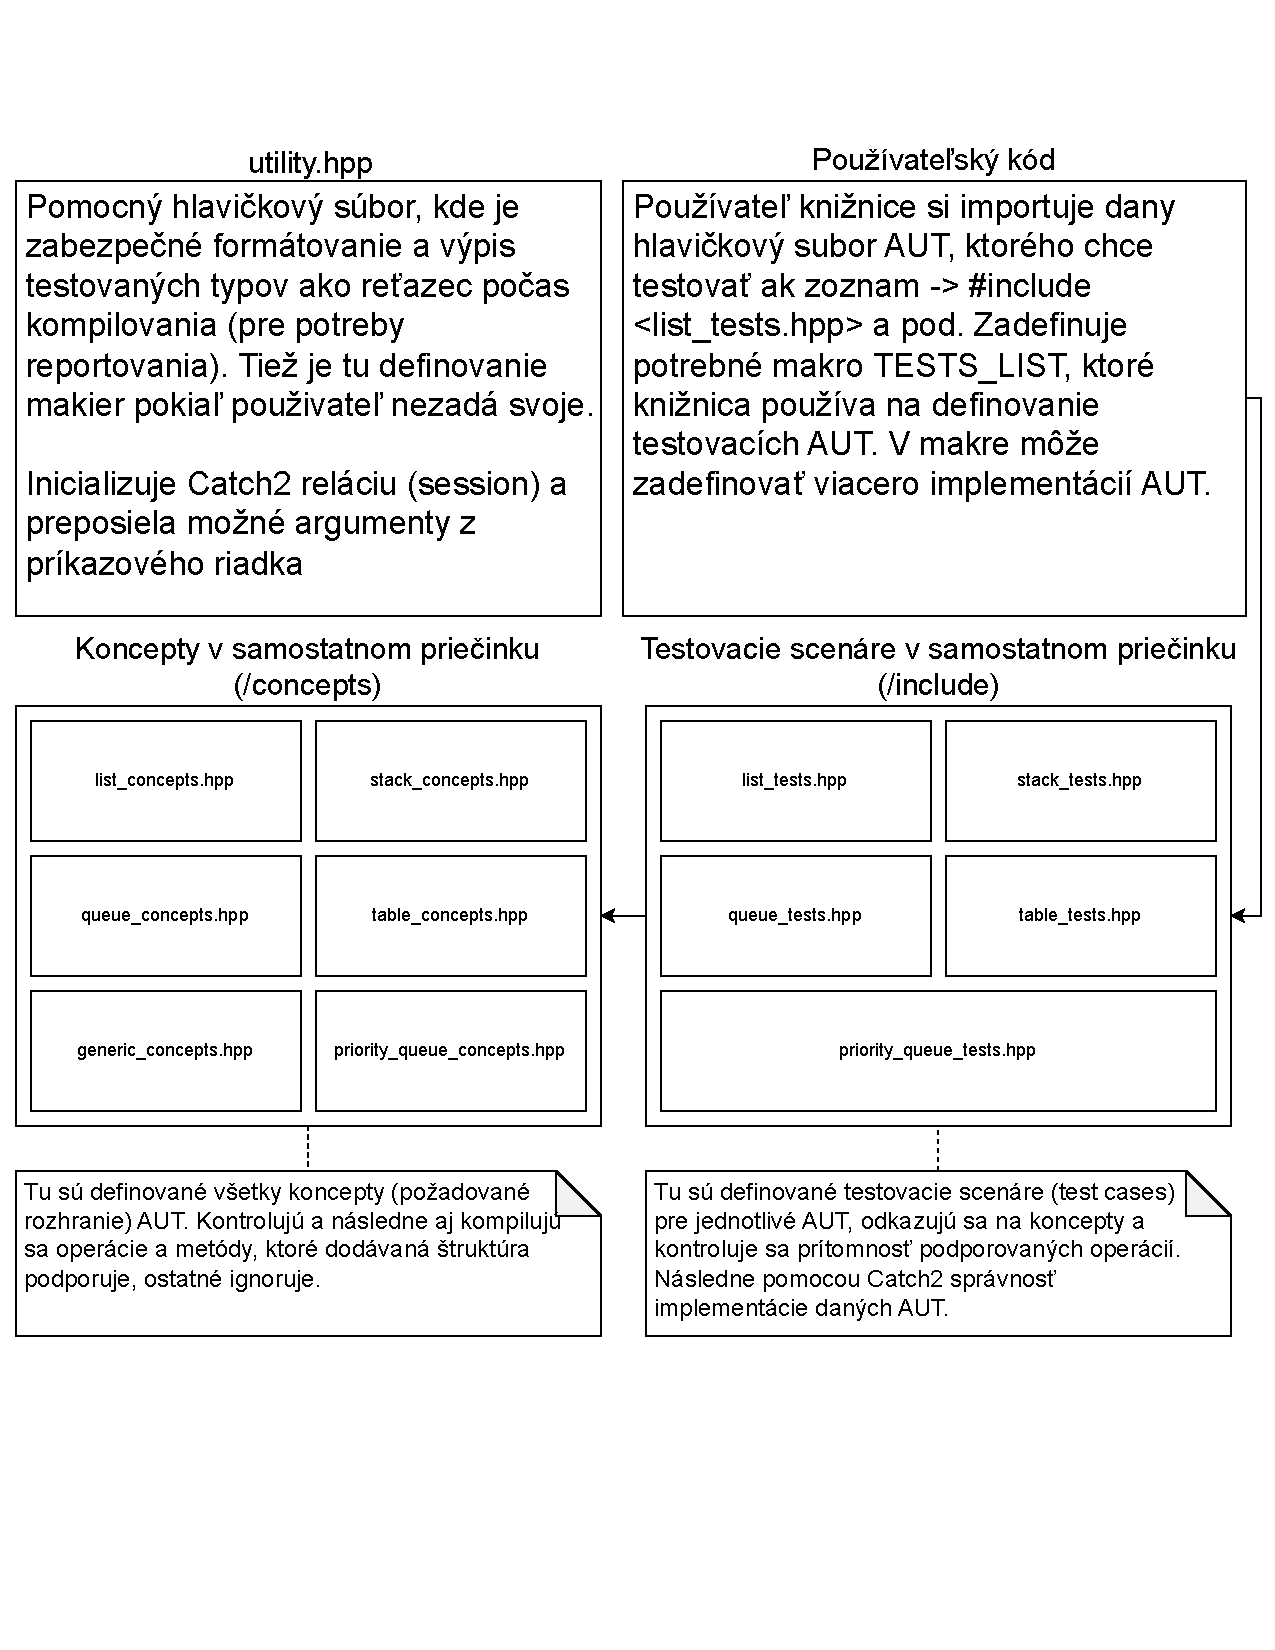
\includegraphics[width=\textwidth]{arch_diagram.pdf}
  }
  \caption{Diagram architektúry knižnice}
  \label{fig:arch_diagram}
\end{figure}

\subsection{Návrh rozhraní a použitie konceptov}

Kľúčovým prvkom návrhu knižnice je definovanie sady C++ Konceptov pre každý podporovaný abstraktný údajový typ (AUT) a jeho relevantné operácie. Tieto koncepty formalizujú požiadavky na rozhranie, ktoré musí testovaná údajová štruktúra spĺňať, aby s ňou mohli pracovať jednotlivé testovacie scenáre. Koncepty sú definované v samostatných hlavičkových súboroch a zoskupené pomocou menných priestorov (namespaces) (napr. generic\_concepts, list\_concepts, queue\_concepts).

Napríklad, pre základné operácie ako zistenie veľkosti alebo vyprázdnenie štruktúry sú definované všeobecné koncepty v súbore generic\_concepts.hpp:

\begin{lstlisting}[caption={Ukážka všeobecných konceptov (generic\_concepts.hpp)}, label={lst:generic_concepts}]
namespace generic_concepts {

template <typename T>
concept has_empty = requires(T structure) {
  { structure.empty() } -> std::convertible_to<bool>;
};

template <typename T>
concept has_size = requires(T structure) {
  { structure.size() } -> std::convertible_to<std::size_t>;
};

template <typename T>
concept has_clear = requires(T structure) {
  { structure.clear() };
};

template <typename T>
concept has_capacity = requires(const T &t) {
  { t.capacity() } -> std::convertible_to<std::size_t>;
};

} // namespace generic_concepts
\end{lstlisting}

Pre špecifické AUT, ako napríklad zoznam (List), sú definované koncepty pre jeho typické operácie v súbore list\_concepts.hpp:
\begin{lstlisting}[caption={Ukážka konceptov pre zoznam (list\_concepts.hpp)}, label={lst:list_concepts}]
namespace list_concepts {

template <typename T>
concept has_push_back = requires(T structure, typename T::value_type value) {
  { structure.push_back(value) };
};

template <typename T>
concept has_at = requires(T structure, std::size_t index) {
  { structure.at(index) } -> std::convertible_to<typename T::value_type>;
};

template <typename T>
concept has_iterator = requires(T structure) {
  typename T::iterator;
  typename T::const_iterator;
  { structure.begin() } -> std::same_as<typename T::iterator>;
  { structure.end() } -> std::same_as<typename T::iterator>;
  { structure.cbegin() } -> std::same_as<typename T::const_iterator>;
  { structure.cend() } -> std::same_as<typename T::const_iterator>;
};

} // namespace list_concepts
\end{lstlisting}

\noindent V tomto súbore sa nachádzajú aj ďalšie koncepty relevantné pre zoznam, ako has\_front, has\_back, has\_remove alebo has\_insert.

Podobne sú definované koncepty pre ďalšie AUT ako front (queue\_concepts.hpp), zásobník (stack\_concepts.hpp), prioritný front (priority\_queue\_concepts.hpp) a tabuľku (table\_concepts.hpp). Tieto koncepty umožňujú testovacím scenárom presne špecifikovať, aké operácie musia byť dostupné, aby sa daný test mohol skompilovať a vykonať. Ak testovaná štruktúra nespĺňa požadovaný koncept, kód testu sa vďaka mechanizmu konceptov ani neskompiluje, čo zabraňuje chybám pri behu.

\subsection{Testovacie scenáre}

Samotné testy sú implementované ako šablónové testovacie prípady pomocou knižnice Catch2, konkrétne s využitím makra TEMPLATE\_LIST\_TEST\_CASE. Toto makro umožňuje spustiť ten istý testovací kód pre rôzne implementácie AUT rovnakého typu. Ktoré konkrétne typy sa budú testovať, definuje používateľ knižnice pomocou makra TESTS\_LIST, ktoré typicky obsahuje std::tuple s konkrétnymi typmi štruktúr.

Selektívna kompilácia jednotlivých častí testu je dosiahnutá pomocou if constexpr v kombinácii s predtým definovanými konceptmi. Tým sa zabezpečí, že sa testujú iba tie operácie, ktoré daná štruktúra skutočne podporuje podľa definovaných konceptov.

Nasledujúca ukážka z list\_tests.hpp demonštruje testovanie operácií prístupu pre AUT zoznam. Šablónový parameter TestType tu reprezentuje jeden z typov definovaných používateľom v makre TESTS\_LIST.

Vypísanie typu pomocou type\_name<TestType>() (z utility.hpp) slúži na informačné účely pri spustení testov.

\begin{lstlisting}[caption={Ukážka testovacieho scenára pre Zoznam (list\_tests.hpp)}, label={lst:list_test_example}]
#include <catch2/catch_template_test_macros.hpp>
#include <concepts/generic_concepts.hpp>
#include <concepts/list_concepts.hpp>
#include <utility.hpp>
#include <iostream>
#include <stdexcept>

TEMPLATE_LIST_TEST_CASE("List access operations",
                        "[list][access]", TESTS_LIST) {
  std::cout << "Testing type: " << type_name<TestType>() << std::endl;

  TestType test_type{5, 4, 10, 41};
  REQUIRE(test_type.size() == 4);

  if constexpr (list_concepts::has_at<TestType>) {
    SECTION("Access") {
      REQUIRE(test_type.at(0) == 5);
      REQUIRE(test_type.at(1) == 4);
      REQUIRE(test_type.at(2) == 10);
      REQUIRE(test_type.at(3) == 41);
    }
  }

  if constexpr (list_concepts::has_front<TestType>) {
    SECTION("Front") {
      REQUIRE(test_type.front() == 5);
    }
  }

  if constexpr (list_concepts::has_back<TestType>) {
    SECTION("Back") {
      REQUIRE(test_type.back() == 41);
    }
  }
}
\end{lstlisting}

V tomto príklade sa kód v rámci prvého if constexpr bloku skompiluje a vykoná iba vtedy, ak aktuálny testovaný typ TestType (vybraný z TESTS\_LIST) spĺňa koncept list\_concepts::has\_at. Podobne sa sekcia testujúca operáciu front vykoná len pre typy spĺňajúce list\_concepts::has\_front a sekcia pre back len pre typy spĺňajúce list\_concepts::has\_back.

Tento prístup zabezpečuje, že knižnica je flexibilná a dokáže testovať širokú škálu implementácií s rôznymi sadami podporovaných operácií, pričom sa kompiluje iba relevantný testovací kód. Podobná štruktúra testov je použitá aj pre ostatné AUT (Front, Zásobník, Prioritný Front, Tabuľka).

\subsection{Technológie pre implementáciu}

Implementácia knižnice bude využívať nasledujúce technológie a nástroje:

\begin{itemize}
  \item \textbf{Jazyk a Štandard:} C++23 pre využitie najnovších prvkov, najmä konceptov.
  \item \textbf{Testovací Framework:} Catch2 v3.x, integrovaný pomocou CMake. Poskytuje základňu pre definíciu, spúšťanie a reportovanie testov. Používajú sa najmä TEMPLATE\_TEST\_CASE\_SIG pre parametrizáciu typov. Aj s možnosťou generovania reportov v rôznych formátoch (XML, JUnit, konzola).
  \item \textbf{Build Systém:} CMake (verzia 3.16 alebo novšia odporúčaná) poskytuje cross-kompiláciu do viacerých operačných systémov ako sú Linux, MacOS a Windows, správu závislostí (Catch2) a definíciu kompilácie, automaticky spravuje závislosti a aktualizácie. Umožňuje jednoduchý setup pre prípadných open-source kolaborantov.
  \item \textbf{Kompilátor:} Primárne Clang (verzia podporujúca C++23), je to moderný kompilátor, ktorý je súčasťou LLVM projektu a podporuje viacero operačných systémov (OS) ako sú: MacOS, Linux a Windows. Disponuje čitateľnejšími chybovými správami oproti MSVC/GCC, v niektorých prípadoch rýchlejšie kompiluje a poskytuje optimalizovaný, resp. efektívnejší beh už skompilovaných programov.
\end{itemize}

Tento návrh poskytuje pevný základ pre implementáciu flexibilnej a robustnej knižnice na testovanie C++ údajových štruktúr. Dôraz na koncepty a adaptačnú vrstvu zabezpečí univerzálnosť a selektívnu kompiláciu, zatiaľ čo využitie Catch2 zjednoduší tvorbu a správu samotných testov.

% --- Implementácia ---
\newpage
\section{Implementácia}

Implementácia knižnice je založená na modulárnom prístupe, ktorý oddeľuje definície požiadaviek (koncepty), testovacie scenáre a nástroje pre používateľa.

\subsection{Štruktúra projektu}

Jadro knižnice tvoria dve hlavné skupiny hlavičkových súborov:

\begin{itemize}
  \item \textbf{Súbory s konceptmi} (concepts/*.hpp): Obsahujú definície C++ Konceptov pre všeobecné vlastnosti údajových štruktúr (generic\_concepts.hpp) a pre špecifické operácie jednotlivých AUT (list\_concepts.hpp, queue\_concepts.hpp, stack\_concepts.hpp, priority\_queue\_concepts.hpp, table\_concepts.hpp). Tieto koncepty formalizujú očakávané rozhranie testovaných štruktúr.
  \item \textbf{Súbory s testovacími scenármi} (tests/*.hpp): Pre každý AUT existuje samostatný súbor (list\_tests.hpp, queue\_tests.hpp, stack\_tests.hpp, priority\_queue\_tests.hpp, table\_tests.hpp), ktorý obsahuje testovacie prípady napísané pomocou frameworku Catch2. Tieto testy sú implementované ako šablóny (TEMPLATE\_LIST\_TEST\_CASE) a využívajú definované koncepty na zabezpečenie selektívnej kompilácie.
\end{itemize}

\noindent Okrem toho knižnica poskytuje pomocné nástroje, ako napríklad funkciu na získanie názvu typu pre výpisy (type\_name v utility.hpp) a štruktúru (struct) data\_type\_probe na spustenie testovacieho procesu.
\begin{lstlisting}[caption={Ukážka inicializácie Catch2 relácie}, label={lst:main}]
#ifndef TESTS_LIST
#pragma message("TESTS_LIST macro not defined. Using default structure: std::vector<int>")
using DefaultTypes = std::tuple<std::vector<int>>;
#define TESTS_LIST DefaultTypes
#endif

struct data_type_probe {
  static int run_tests(int argc, char *argv[]) {
    Catch::Session session;

    // Apply any command line arguments to Catch2
    int return_code = session.applyCommandLine(argc, argv);

    // Indicates a command line error
    if (return_code != 0) {
      return return_code;
    }

    // Run the Catch2 session, which will run the test cases
    int result = session.run();

    return result;
  }
};
\end{lstlisting}
\noindent Štruktúra (struct) data\_type\_probe (\hyperref[lst:main]{Zdrojový kód: \ref*{lst:main}}) je zodpovedná za inicializáciu a spustenie testovacej relácie Catch2. Súčasťou utility.hpp je aj mechanizmus, ktorý zabezpečí predvolenú definíciu makra TESTS\_LIST (s typom std::vector<int>), ak ho používateľ sám nedefinuje pred zahrnutím hlavičkových súborov knižnice.

\subsection{Testovanie používateľskej štruktúry}
\label{subsec:princip_fungovania}

Fungovanie knižnice je postavené na spolupráci C++ šablón, C++ konceptov a testovacieho frameworku Catch2. Proces testovania používateľom dodanej štruktúry prebieha nasledovne:

\begin{enumerate}
\item \textbf{Definícia testovaných typov:} Používateľ vo svojom kóde (napr. v hlavnom súbore projektu, ako ukazuje \hyperref[lst:example_types]{príklad v Zdrojovom kóde \ref*{lst:example_types}}) definuje, ktoré konkrétne typy údajových štruktúr chce testovať. Robí tak pomocou definície makra TESTS\_LIST, ktorému typicky priradí std::tuple obsahujúci zoznam typov. Môže ísť o štruktúry zo štandardnej knižnice (napr. std::vector<int>, std::map<int, int>), vlastné implementácie (napr. custom\_vec<int>), alebo adaptéry obaľujúce tieto štruktúry, ak je potrebné prispôsobiť ich rozhranie.
\begin{lstlisting}[label={lst:example_types}]
using MyTypes = std::tuple<std::queue<int>>;
#define TESTS_LIST MyTypes
\end{lstlisting}
\item \textbf{Zahrnutie testovacích sád:} Používateľ následne zahrnie (\#include) hlavičkové súbory s testovacími scenármi pre tie AUT, ktoré chce testovať (list\_tests.hpp, queue\_tests.hpp, atď.).
\begin{lstlisting}[label={lst:example_includes}]
#include <queue_tests.hpp>
\end{lstlisting}
\item \textbf{Inštanciácia šablónových testov:} Keď kompilátor spracuje zahrnutý súbor s testami (napr. queue\_tests.hpp), narazí na makro TEMPLATE\_LIST\_TEST\_CASE. Toto makro z knižnice Catch2 automaticky expanduje testovací kód pre každý typ uvedený v makre TESTS\_LIST. Pre každý takýto typ sa vytvorí inštancia testovacieho prípadu, kde šablónový parameter (v kóde knižnice typicky pomenovaný TestType) je nahradený konkrétnym typom z TESTS\_LIST.
\item \textbf{Selektívna kompilácia pomocou konceptov:} Vnútri kódu testovacieho prípadu sa rozsiahlo využíva konštrukcia if constexpr v spojení s C++ konceptmi definovanými v concepts/*.hpp. Každá časť testu, ktorá overuje špecifickú operáciu (napr. push, pop, at, contains), je podmienená splnením príslušného konceptu pre aktuálny TestType.
\begin{lstlisting}[caption={Použitie if constexpr a konceptov v teste (queue\_tests.hpp)}, label={lst:if_constexpr_example}]
if constexpr (queue_concepts::has_push<TestType> &&
              queue_concepts::has_pop<TestType> &&
              generic_concepts::has_size<TestType>) {
  SECTION("Push and Pop Operations (FIFO Verification)") {
    // ...
    REQUIRE_NOTHROW(test_queue.push(1));
    REQUIRE(test_queue.pop() == 1);
    // ...
  }
}
if constexpr (queue_concepts::has_front_queue<TestType>) {
  SECTION("Front Access") {
    // ...
  }
}
\end{lstlisting}

Ak TestType spĺňa daný koncept (t.j. poskytuje požadovanú metódu so správnou signatúrou a návratovým typom), blok kódu vnútri if constexpr je ponechaný a skompilovaný. Ak TestType koncept nespĺňa, celý blok kódu je počas kompilácie odstránený (discarded). Toto zabezpečuje, že sa pre danú štruktúru kompilujú a následne spúšťajú len tie testy, ktoré sú pre ňu relevantné a ktorých operácie podporuje.

\item \textbf{Spustenie testov v kóde:} Nakoniec používateľ vo svojej funkcii main zavolá statickú metódu data\_type\_probe::run\_tests(argc, argv). Táto metóda inicializuje a spustí testovaciu reláciu frameworku Catch2, ktorý automaticky objaví a vykoná všetky skompilované testovacie prípady a vypíše výsledky.
\end{enumerate}

Tento mechanizmus umožňuje knižnici poskytovať jednotnú sadu testov pre rôzne implementácie AUT, pričom sa automaticky prispôsobuje schopnostiam každej konkrétnej testovanej štruktúry vďaka sile C++ konceptov a šablónového metaprogramovania. Výsledkom je flexibilný a robustný systém testovania s jasnou spätnou väzbou už počas kompilácie v prípade nekompatibilného rozhrania testovanej štruktúry.

\subsection{Implementačné výzvy}

Počas implementácie knižnice bolo potrebné riešiť niekoľko výziev:
\begin{itemize}
  \item \textbf{Heterogenita API:} Rôzne implementácie (aj v rámci STL) môžu mať mierne odlišné názvy metód, návratové typy alebo sémantiku pre rovnakú operáciu. Návrh konceptov musel byť dostatočne flexibilný, aby pokryl bežné variácie, alebo by si vyžadoval použitie adaptačných tried pre neštandardné rozhrania.
  \item \textbf{Definícia konceptov:} Správne definovanie konceptov tak, aby presne zachytávali požadované vlastnosti bez zbytočných obmedzení, si vyžadovalo starostlivé zváženie. Napríklad koncept pre iterátory (list\_concepts::has\_iterator, table\_concepts::has\_iterator) musí overiť existenciu typov iterator, const\_iterator a metód begin(), end(), cbegin(), cend() s korektnými návratovými typmi.
  \item \textbf{Spracovanie chýb a výnimiek:} Testy musia overovať aj správanie pri chybných vstupoch (napr. prístup mimo rozsahu v at(), volanie pop() na prázdnej štruktúre). V testoch sa na to používajú makrá Catch2 ako REQUIRE\_THROWS\_AS (viditeľné napr. v list\_tests.hpp). Koncepty samotné však typicky neoverujú sémantiku spracovania chýb, to zostáva úlohou samotných testovacích scenárov.
  \item \textbf{Zabezpečenie správnej selektívnej kompilácie:} Bolo nutné dôsledne používať if constexpr s konceptmi vo všetkých relevantných častiach testovacích scenárov, aby sa predišlo kompilačným chybám pri testovaní štruktúr, ktoré nepodporujú všetky testované operácie.
\end{itemize}

\subsection{Použitie CMake na zostavenie knižnice}

Projekt využíva systém CMake na správu procesu kompilácie a závislostí. Hlavný konfiguračný súbor CMakeLists.txt definuje samotnú knižnicu ako INTERFACE knižnicu (keďže je primárne header-only), nastavuje požadovaný štandard C++23 a spravuje závislosti. Kľúčovou závislosťou je testovací framework Catch2, ktorý sa získava automaticky pomocou CMake modulu FetchContent priamo z Git repozitára.

Pre demonštráciu použitia knižnice slúži samostatný konfiguračný súbor (v príklade CMakeLists\_example.txt), ktorý ukazuje, ako používateľský projekt definuje spustiteľný súbor (napr. example\_usage z example.cpp) a prepojí ho s našou knižnicou DataTypeProbe. Tým získa prístup k jej hlavičkovým súborom (konceptom, testom, utilitám) a prepojenie na Catch2.

\subsection{Formátovanie kódu pomocou clang-format}

Pre zabezpečenie jednotného a konzistentného štýlu formátovania zdrojového kódu v celom projekte sa využíva nástroj clang-format. Tento nástroj automaticky upravuje formátovanie C++ kódu podľa preddefinovaných pravidiel. Konfigurácia pre tento projekt je uložená v súbore .clang-format a vychádza zo štýlu LLVM, ktorý je populárny v C++ komunite.

\noindent Použitie nástroja clang-format prináša niekoľko výhod:

\begin{itemize}
  \item \textbf{Konzistentnosť:} Všetok kód dodržiava rovnaké pravidlá formátovania, bez ohľadu na autora alebo použité IDE.
  \item \textbf{Čitateľnosť:} Jednotný štýl uľahčuje čítanie a pochopenie kódu.
  \item \textbf{Zníženie "šumu" pri revíziách kódu:} Zmeny sa týkajú logiky, nie formátovania.
  \item \textbf{Podpora kolaborácie:} V prípade open-source projektu alebo tímovej práce odstraňuje nezhody ohľadom štýlu a zjednodušuje integráciu kódu od rôznych prispievateľov.
\end{itemize}

\subsection{Open-Source aspekt a podpora kolaborácie}

Ako je uvedené \hyperref[priloha:b]{v Prílohe~\ref*{priloha:b}} a \hyperref[priloha:c]{Prílohe~\ref*{priloha:c}}, knižnica aj samotná bakalárska práca sú vyvíjané s úmyslom zverejnenia ako open-source projekty na platforme GitHub. Tento prístup je podporený použitím nástrojov a praktík, ktoré uľahčujú externú spoluprácu a ďalší rozvoj komunitou:

\begin{itemize}
  \item \textbf{CMake:} Poskytuje štandardizovaný a multiplatformový build systém. Ktokoľvek si môže projekt stiahnuť a skompilovať pomocou bežných CMake postupov bez potreby špecifických nastavení pre konkrétne prostredie.
  \item \textbf{Clang-Format:} Zabezpečuje jednotný kódovací štýl. Vývojári môžu ľahko formátovať svoj kód podľa projektových štandardov, čím sa predchádza nekonzistenciám a uľahčujú sa revízie kódu (code reviews).
  \item \textbf{GitHub:} Platforma poskytuje nástroje pre verzovanie kódu (Git), sledovanie problémov (Issues), navrhovanie zmien (Pull Requests) a diskusiu, čo sú základné piliere pre spoluprácu na open-source projektoch.
  \item \textbf{Licencia MIT:} Výber voľnej licencie ako MIT umožňuje široké použitie, modifikáciu a distribúciu knižnice.
\end{itemize}

Kombinácia týchto technológií a zvolenej platformy vytvára prostredie priaznivé pre transparentný vývoj, jednoduchú adopciu knižnice a potenciálnu kolaboráciu s externými vývojármi v rámci open-source komunity.

\subsection{Návod na otestovanie vlastnej štruktúry}

Používateľ, ktorý chce otestovať vlastnú implementáciu údajovej štruktúry pomocou tejto knižnice, by mal postupovať nasledovne:

\begin{enumerate}
\item \textbf{Pripraviť projekt:} Stiahnuť zdrojové kódy knižnice (napr. z GitHub repozitára). Nastaviť CMake projekt podľa vzoru v CMakeLists\_example.txt alebo integrovať knižnicu do existujúceho projektu. Uistiť sa, že je dostupná knižnica Catch2 (CMake by ju mal stiahnuť automaticky).
\item \textbf{Implementovať štruktúru:} Vytvoriť vlastnú triedu údajovej štruktúry (napr. MyList<T>). Dôležité je, aby metódy tejto triedy zodpovedali názvom a signatúram očakávaným konceptmi pre daný AUT (napr. pre zoznam by mala mať metódy ako push\_back, size, empty, at, begin, end atď., ak majú byť testované príslušnými konceptmi). Ak rozhranie nezodpovedá, je potrebné vytvoriť adaptačnú triedu.
\item \textbf{Definovať testované typy:} V hlavnom spustiteľnom súbore (napr. main.cpp alebo example.cpp) definovať makro TESTS\_LIST ako std::tuple obsahujúci typ (alebo typy), ktoré sa majú testovať.
\begin{lstlisting}
#include "MojaStruktura.hpp"
#include <vector>

using MyTypes = std::tuple<MyList<int>, std::vector<int>>;
#define TESTS_LIST MyTypes
\end{lstlisting}
\item \textbf{Zahrnúť testy:} Zahrnúť hlavičkové súbory s testovacími scenármi pre požadované AUT.
\begin{lstlisting}
#include <list_tests.hpp> // Zahrnie testy pre AUT Zoznam
\end{lstlisting}
\item \textbf{Spustiť testy:} Vytvoriť funkciu main a zavolať v nej data\_type\_probe::run\_tests(argc, argv).
\begin{lstlisting}
#include <utility.hpp>

int main(int argc, char *argv[]) {
  int result = data_type_probe::run_tests(argc, argv);
  return result;
}
\end{lstlisting}
\item \textbf{Skompilovať projekt:} Skompilovať projekt pomocou CMake.
\item \textbf{Spustiť a filtrovať testy:} Spustiť výsledný spustiteľný súbor (executable). Catch2 automaticky vykoná všetky relevantné testy pre definované typy a vypíše výsledky.
  \begin{itemize}
    \item \textbf{Filtrovanie pomocou tagov:} Testovacie prípady v knižnici sú označené značkami (tagmi) v hranatých zátvorkách, napríklad [list], [access], [basic], [queue]. Tieto tagy umožňujú spustiť iba vybranú podmnožinu testov pomocou argumentov príkazového riadku, napríklad:
    \begin{itemize}
      \item Spustenie iba testov pre Zoznam: \lstinline|./nazov_programu [list]|
      \item Spustenie iba testov prístupových metód Zoznamu: \lstinline|./nazov_programu [list][access]|
      \item Vypísanie všetkých dostupných tagov: \lstinline|./nazov_programu --list-tags|
    \end{itemize}
    Táto funkcionalita Catch2 umožňuje používateľovi efektívne zamerať testovanie na konkrétne časti alebo aspekty implementácie.
  \end{itemize}
\end{enumerate}

Knižnica bola navrhnutá tak, aby bola čo najjednoduchšie použiteľná. Používateľ typicky potrebuje len zahrnúť potrebné hlavičkové súbory, zadefinovať svoju údajovú štruktúru a typy v makre TESTS\_LIST a spustiť testy. Komplexnosť overovania rozhrania a selektívnej kompilácie je z veľkej časti skrytá v mechanizme konceptov a šablónových testov.

% --- Vyhodnotenie ---
\newpage
\section{Vyhodnotenie} \label{sec:vyhodnotenie}

Táto kapitola sa zameriava na praktické overenie a vyhodnotenie vlastností implementovanej testovacej knižnice. Hlavným cieľom bolo overiť kľúčovú funkcionalitu selektívnej kompilácie pomocou C++ konceptov a jej vplyv na čas kompilácie. Ďalej sme hodnotili úspešnosť a komplexnosť testov pri odhaľovaní chýb v implementáciách údajových štruktúr.

\subsection{Overenie selektívnej kompilácie a vplyv na čas kompilácie}

Jedným z hlavných prínosov použitia C++ konceptov v spojení s if constexpr je možnosť selektívnej kompilácie testov. Očakávali sme, že ak testovaná údajová štruktúra implementuje iba podmnožinu operácií definovaných konceptmi pre daný AUT, čas kompilácie testovacieho projektu bude kratší, pretože kompilátor nebude musieť generovať kód pre neaplikovateľné testovacie sekcie.

\noindent Na overenie tohto predpokladu sme vykonali sériu meraní času kompilácie pre rôzne scenáre:

\begin{enumerate}
    \item \textbf{Referenčný scenár:} Testovanie vlastnej implementácie zoznamu (len wrapper okolo std::vector).
    \item \textbf{Scenár s minimalizovanou štruktúrou:} Testovanie vlastnej, minimalistickej implementácie zoznamu (custom\_vec), ktorá implementuje iba základné operácie push\_back a pop\_back, a chýbajú jej ostatné operácie.
\end{enumerate}

Merania času kompilácie boli vykonané opakovane za rovnakých podmienok (rovnaký hardvér, operačný systém, verzia kompilátora Clang, vypnuté paralelné kompilovanie, čistenie build adresára pred každým meraním) pre oba scenáre. Vybrali sme počet replikácií sto. Sledovali sme celkový čas potrebný na skompilovanie projektu obsahujúceho definíciu príslušného typu v TESTS\_LIST a zahrnutie súboru list\_tests.hpp. Tu sa preukáže aj odolnosť knižnice voči zmenám v implementácii, knižnica nepadne pri behu, ak sa zmení rozhranie testovanej štruktúry. Len sa dané testy neimplementovaných operácií preskočia.

\begin{figure}[H]
    \centering
    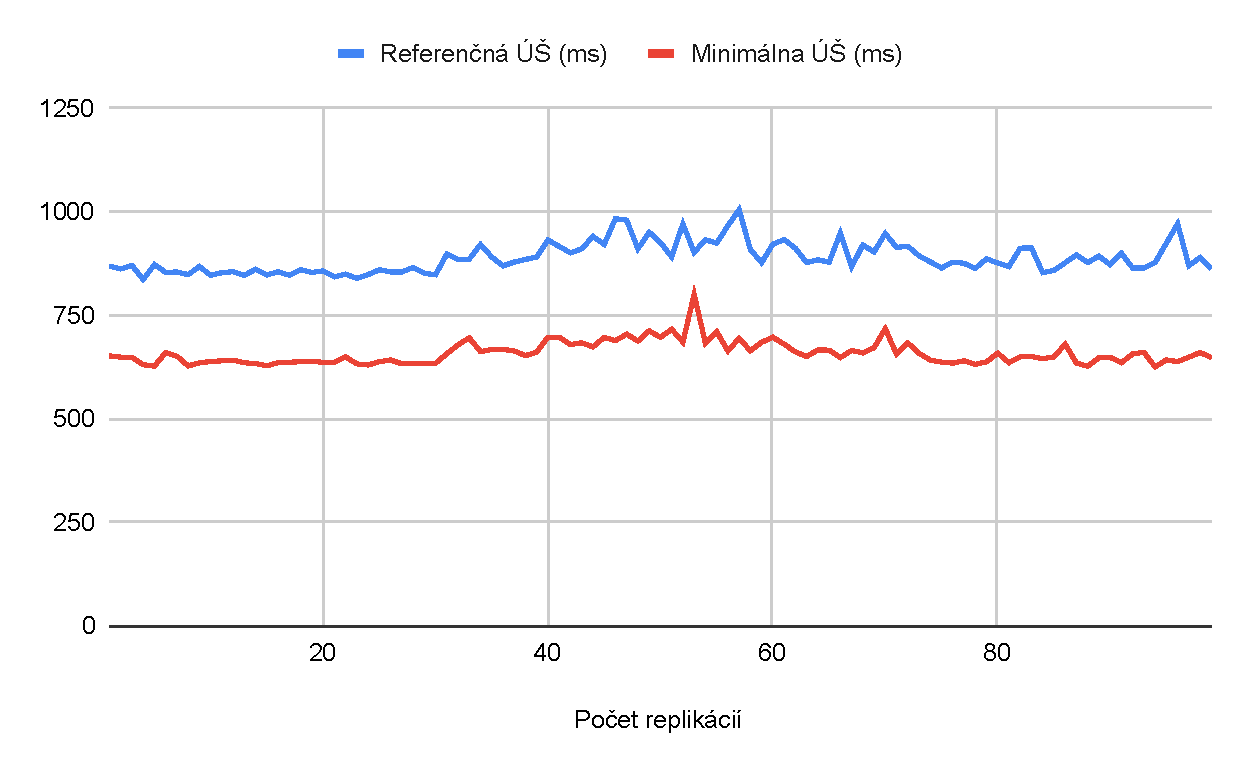
\includegraphics[width=\textwidth]{compilation_time.pdf}
    \caption{Porovnanie časov kompilácie (x: Počet replikácií, y: Čas kompilácie [ms])}
    \label{fig:kompilacia_cas}
\end{figure}

Výsledky sme museli spracovať, t.j. odstránenie extrémnych odchýlok a vypočítali sme priemerné časy kompilácie. Nakoniec na \hyperref[fig:kompilacia_cas]{Obrázku \ref*{fig:kompilacia_cas}}, môžeme potvrdiť očakávania. Kompilácia projektu testujúceho custom\_vec<int> bola merateľne rýchlejšia v porovnaní s kompiláciou testov pre plne vybavený custom\_vec<int> (obalený std::vector). Priemerný čas kompilácie minimálnej štruktúry bol: 658.97 ms naopak referenčnej 888.64 ms, čo činí priemerné urýchlenie kompilácie minimálnej štruktúry o 29.68\%. Toto vylepšenie pripisujeme práve mechanizmu selektívnej kompilácie -- kompilátor preskočil časti testovacieho kódu v list\_tests.hpp, ktoré boli podmienené konceptmi nespĺňanými štruktúrou custom\_vec<int>. Aj keď absolútny rozdiel v čase nemusí byť dramatický pre malý projekt s jedným testovaným typom, pri rozsiahlejších projektoch s viacerými testovanými štruktúrami alebo komplexnejšími testovacími sadami môže tento efekt prispieť k citeľnému zrýchleniu celkového build procesu. Potvrdzuje to efektivitu použitia konceptov na optimalizáciu kompilácie v kontexte testovania heterogénnych implementácií.

\subsection{Odhaľovanie chýb v implementáciách}

Ďalším aspektom hodnotenia bola schopnosť navrhnutých testovacích scenárov odhaliť bežné chyby v implementáciách údajových štruktúr. Na tento účel sme pripravili niekoľko zámerne chybných verzií jednoduchých údajových štruktúr zoznam s "off-by-one" chybou pri prístupe cez index. Následne sme tieto chybné implementácie otestovali pomocou našej knižnice zahrnutím príslušných testovacích sád (list\_tests.hpp).

\begin{figure}[H]
    \centering
    \lstset{style=barebones}
    \begin{lstlisting}
$ ./tests/example_usage -r compact
RNG seed: 2054445050
Testing type: custom_vec<int>
DataTypeProbe/include/list_tests.hpp:21: failed: test_type.at(0) == 5 for: 4 == 5
DataTypeProbe/include/list_tests.hpp:129: failed: test_type.at(0) == 1 for: 4 == 1
DataTypeProbe/include/list_tests.hpp:226: failed: copy.at(0) == 1 for: 2 == 1
DataTypeProbe/include/list_tests.hpp:235: failed: assigned.at(0) == 4 for: 5 == 4
DataTypeProbe/include/list_tests.hpp:244: failed: list.at(0) == 1 for: 2 == 1
DataTypeProbe/include/list_tests.hpp:255: failed: original.at(0) == 1 for: 2 == 1
DataTypeProbe/include/list_tests.hpp:271: failed: assigned.at(0) == 7 for: 8 == 7
test cases:  16 |  11 passed | 5 failed
assertions: 118 | 109 passed | 9 failed
    \end{lstlisting}
    \caption{Ukážka výstupu pri detekcii chyby v testovanej štruktúre (konzolový výstup)}
    \label{fig:catch2_vystup}
\end{figure}

Vo všetkých pripravených prípadoch testy úspešne identifikovali chyby. Framework Catch2 poskytol jasné a informatívne výstupy (\hyperref[fig:catch2_vystup]{Obrázok \ref*{fig:catch2_vystup}}), ktoré presne lokalizovali zlyhanú aserciu -- chybná implementácia operácie at (off-by-one chyba), zobrazili porovnávané hodnoty (očakávanú vs. skutočnú) a poskytli kontext (názov testovacieho prípadu, typ a sekcie). Toto potvrdzuje, že navrhnuté testovacie scenáre pokrývajú základné funkčné požiadavky a hraničné prípady dostatočne na to, aby odhalili bežné implementačné nedostatky.

\subsection{Zhrnutie výsledkov}

Vyhodnotenie potvrdilo kľúčové prednosti navrhovanej knižnice:

\begin{itemize}
    \item \textbf{Efektívna selektívna kompilácia:} Použitie C++ konceptov skutočne vedie k optimalizácii času kompilácie pri testovaní štruktúr s obmedzeným rozhraním.
    \item \textbf{Detekcia chýb:} Implementované testovacie scenáre sú schopné identifikovať bežné chyby v logike údajových štruktúr.
    \item \textbf{Informatívnosť:} Integrácia s Catch2 poskytuje jasné a užitočné reporty o výsledkoch testov a prípadných zlyhaniach.
\end{itemize}

\noindent Tieto výsledky naznačujú, že knižnica spĺňa svoje hlavné ciele a predstavuje funkčný a prakticky použiteľný nástroj na testovanie údajových štruktúr v C++.

% --- Záver ---
\newpage
\section*{Záver}
\addcontentsline{toc}{section}{\protect\numberline{}Záver}
Výsledkom tejto bakalárskej práce je návrh a implementácia univerzálnej testovacej knižnice v jazyku C++, ktorá predstavuje efektívny nástroj na validáciu implementácií základných abstraktných údajových typov. Kľúčovou vlastnosťou knižnice je jej schopnosť pracovať s rôznymi C++ implementáciami (zo STL, Boostu, alebo vlastnými) prostredníctvom jednotného testovacieho rozhrania a adaptačnej vrstvy. Využitím moderných C++ prvkov, predovšetkým konceptov (C++20/23), knižnica zabezpečuje selektívnu kompiláciu testov -- kompilujú a spúšťajú sa len tie testy, ktorých požiadavky na operácie testovaná štruktúra spĺňa. Tým sa zvyšuje efektivita a relevantnosť testovacieho procesu.

Návrh knižnice kládol dôraz na modularitu a rozšíriteľnosť, čo umožňuje v budúcnosti jednoducho pridávať nové testovacie scenáre alebo podporu pre ďalšie abstraktné údajové typy. Použitie etablovaného testovacieho frameworku Catch2 poskytuje robustný základ pre vykonávanie testov a generovanie prehľadných reportov. Multiplatformová kompatibilita zabezpečená použitím CMake a štandardného C++ ďalej zvyšuje použiteľnosť knižnice v rôznych vývojových prostrediach (Linux, macOS, Windows).

Táto práca úspešne demonštrovala, ako je možné skombinovať teoretické znalosti o údajových štruktúrach s modernými softvérovými inžinierskymi praktikami (testovanie, generické programovanie, návrhové vzory) na vytvorenie praktického nástroja. Veríme, že výsledná knižnica má potenciál byť cennou pomôckou nielen v akademickej sfére pri výučbe a overovaní študentských prác, ale aj pre C++ vývojárov v praxi, ktorí potrebujú systematicky overovať správnosť vlastných alebo knižničných implementácií údajových štruktúr. Práca zároveň otvorila dvere pre ďalší rozvoj. Budúce smerovanie projektu by sa mohlo zamerať na:

\begin{itemize}
  \item Rozšírenie sady testov o komplexnejšie scenáre a testovanie invariantov.
  \item Implementáciu výkonnostných testov.
  \item Zlepšenie používateľského rozhrania a dokumentácie.
  \item Presadiť knižnicu ako open-source projekt s cieľom prilákať komunitu a podporiť jej ďalší vývoj.
\end{itemize}

Celkovo táto práca predstavuje solídny základ pre nástroj, ktorý môže významne prispieť k zvyšovaniu kvality a spoľahlivosti softvéru využívajúceho základné údajové štruktúry v jazyku C++.

% --- Bibliografia ---
\printbibliography[title={Zoznam použitej literatúry}]

% --- Prílohy ---
\appendix

\newpage
\section*{Príloha A: USB kľúč}
\label{priloha:a}

Na konci bakalárskej práce je pripnutý USB kľúč na ktorom sa nachádzajú všetky súbory potrebné na spustenie knižnice a testovacej aplikácie, vrátane elektronickej podoby tejto bakalárskej práce.

\noindent Obsahuje:

\begin{itemize}
  \item Zdrojový kód knižnice
  \item CMake konfiguračné súbory
  \item README súbor s inštrukciami na spustenie
  \item Príklady použitia knižnice
  \item Elektronickú verziu bakalárskej práce (vo formáte PDF)
\end{itemize}

\newpage
\section*{Príloha B: Online distribúcia zdrojového kódu}
\label{priloha:b}

% Assuming use of url or hyperref package for \url
Zdrojový kód knižnice vyvinutej v rámci tejto bakalárskej práce je dostupný vo verejnom repozitári na platforme GitHub na adrese: \url{https://github.com/Viro102/DataTypeProbe}, repozitár obsahuje kompletný zdrojový kód knižnice, konfiguračné súbory CMake, príklady použitia a programátorskú dokumentáciu (v podobe README).

\newpage
\section*{Príloha C: Online distribúcia zdrojového kódu tohto dokumentu (LaTeX)}
\label{priloha:c}

Zdrojový kód tohto dokumentu je voľne dostupný v repozitári na platforme GitHub na adrese: \url{https://github.com/Viro102/bachelor_thesis}, aj odkazom ku GitHub repozitáru v prílohe \ref{priloha:b} pomocou GitHub submodulu.

\end{document}
